\documentclass[openany]{article}
\usepackage{graphicx}
\usepackage{float}
\usepackage[colorlinks]{hyperref}
\graphicspath{{Illustrations/} {Illustrations/Website/}}

\title{\textbf{COMP1044 Coursework Assignment 2 Final Report} \\ Group 15 / Chew Language}
\author{
	Leong Chang Yung, 20307078
	\and
	Lucas Dylan Purnell, 20197316
	\and
	Tan Zhun Xian, 20313854
	\and
	Chong Hao Wei, 20194465
	\and
	Morhaf Allababidi, 20195867
	\and
	Thomas Tan Kean Yew, 20316601
}
\date{\today}

\begin{document}
\maketitle
\newpage
\tableofcontents
\newpage

\section{Report Part A}
\subsection{Entity Relation Diagram, 1st Iteration}
	\begin{figure}[H]
		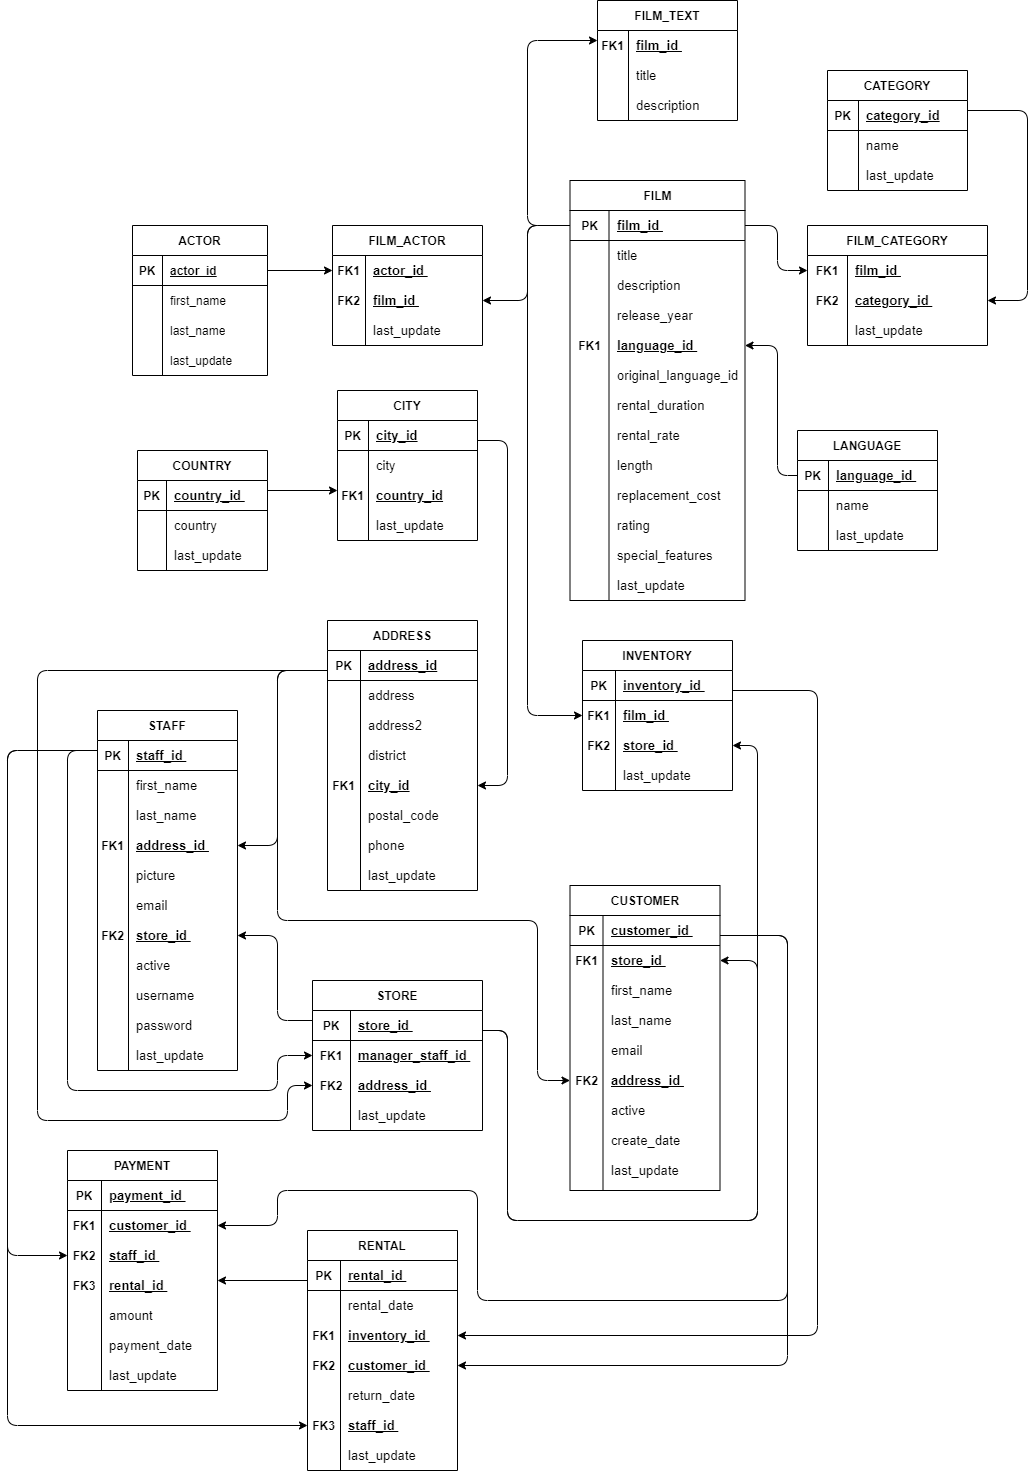
\includegraphics[width=\textwidth]{DBICourseworkA}
		\caption{Proposed model for database.}	
	\end{figure}
	\rule{\textwidth}{0.4pt}
		
\subsection{Datatype Selection}
	For every field we chose the datatype depending on what would both match the data we had available and take up the lowest amount of memory possible 
	while still ensuring that the type and length would be suitable for all new entries. 
	\\\\
	For most of the fields that were purely filled with numbers we set the type to either \textbf{int} or \textbf{decimal} (depending on whether the number was an integer 
	or a decimal). A few examples of this are the \emph{id} fields and the \emph{length} and \emph{rating} field in the \emph{film} table. A notable exception to this was the 
	\emph{phone number} field. We set this datatype to \textbf{varchar} to allow people to enter their phone numbers in a different format despite all phone numbers in the 
	dataset being integers. This was because many phone numbers need either a plus or a dash. Additionally, this field could be parsed and converted into an integer later if needed.
	\\\\	
	For all \textbf{varchar} we used the same principle but for the majority of fields we tried to keep the maximum lengths in neat values (normally multiples of 5). For instance, common 
	values for the maximum length of \textbf{varchar} are 10, 25 and 50. We decided to set each field’s maximum length to the longest realistic input value.
	For instance, we set \emph{film\textunderscore title} to \textbf{varchar(100)} as the longest name for a popular movie was 76 characters. We also set \emph{first\textunderscore name} and 
	\emph{last\textunderscore name} to 50 as we thought that would be a good estimate based on actual estimates of the longest person names.
	\\\\
	All date values were set to the type \textbf{datetime} according to their date and time content. For instance the \emph{last\textunderscore update} and
	\emph{create\textunderscore date} fields.	
	\\
	\rule{\textwidth}{0.4pt}
	
\subsection{Reasoning for Primary and Foreign Key Choice}
	When we were deciding on what to pick for the primary key for each time we understood that it had to be both unique and non-null. 
	This is because the primary key serves as the identifier for each record in the table and if it is either repeated or \textsc{null} it can no longer serve as an identifier. 
	The obvious candidate here was  the ID field in every table (for instance the \emph{inventory\textunderscore id} in the inventory table) as it fulfils both of these criteria.
	\\\\
	The foreign key has the same requirements except that it need not be unique – only the primary key it references has to be unique. 
	With the in mind we can use the same fields that we used as primary keys. Therefore for each of our arrays the \emph{id} column is used to link the tables together. 
	For instance, \emph{customer\textunderscore id} was chosen as the foreign key to link the \emph{payment} table with the \emph{customer} table and \emph{address\textunderscore id} 
	was chosen as the foreign key to link the \emph{staff} table with the \emph{address} table.
	\\
	\rule{\textwidth}{0.4pt}

\subsection{Completeness of the Dataset}
	The database was relatively complete and we did not struggle with the quality of the data. We found that the data values were consistent across the different tables. This meant
	 that we didn’t run into any issues regarding the foriegn keys and we didn’t find conflicting information in the data set.
	\\\\
	We found a few different ways that the dataset was incomplete. The first was missing numbers from the auto-incremental data. For instance,
	 there were missing \emph{address\textunderscore id}’s in \emph{Address.csv}. This problem was easily remedied by enabling the property to \textbf{auto increment} during the creation of said file. 
	\\\\
	The next problem was
	 that many \textsc{null} fields were invalid and are supposed to contain a value. 
	For instance, some of the fields of \emph{Rental\textunderscore id} in \emph{Payment.csv} were \textsc{null} when this should not have been the case. This is a problem as it 
	may compromise the integrity
	 of the database, as these \textsc{null} fields will lead to orphaned records due to the lack of a foriegn key.
	\\\\
	There was also a \textsc{null} value in the \emph{password} column of the \emph{staff.csv} table. This would indicate data corruption, data loss, or staff negligence in inputting a proper password. In the interest of system security, the best remedy would be to get the relevant staff member to provide a value for this \textsc{null} field. However, while the problem stands, we decided that it would be better to leave these fields as \textsc{null} to avoid risking data integrity.
	\\
	\rule{\textwidth}{0.4pt}

\subsection{Errors in the Database}
	We also noticed that in \emph{country.csv} and \emph{customer.csv} that there wasn’t a consistent delimiter. The file alternated between using commas 
	and semicolons to separate data. The lack of support for semicolon delimiters made it impossible to import the data into the database while keeping it in its intended format. 
	To remedy this we replaced the semicolons with commas wherever applicable using text editors.
	\\\\
	While studying the dataset, we discovered that some of the entries have been duplicated, such as the occurrence of two film descriptions in \emph{film\textunderscore text.csv} and \emph{film.csv}. We can resolve this redundancy by removing a duplicate description field on one of the files.
	\\\\
	Another error was the existence of a corrupted picture file within \emph{staff.csv}. This corruption made it impossible to view or display the aforementioned picture. 
	We decided that leaving a corrupted picture within the staff database was not of high importance and wouldn’t decrease the completeness or understandability of the dataset,
	so we just removed the picture. A partial solution was found in making the field type storing the picture as \textbf{longblob}. 
	\begin{figure}[H]
		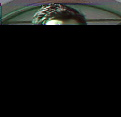
\includegraphics[width=13cm]{staff-picture}
		\caption{The partially recovered staff photo.}
	\end{figure}
	This allowed the picture to be imported, albeit still in an incomplete state. 
	\\
	\rule{\textwidth}{0.4pt}

\subsection{Conclusion}
	At the point of writing, the team determined the database to be sufficient for further usage, due to SELECT queries functioning properly when used to select specific rows in the tables.

\newpage

\section{Report Part B}
\subsection*{Entity Relation Diagram (For Reference)}
	\begin{figure}[H]
		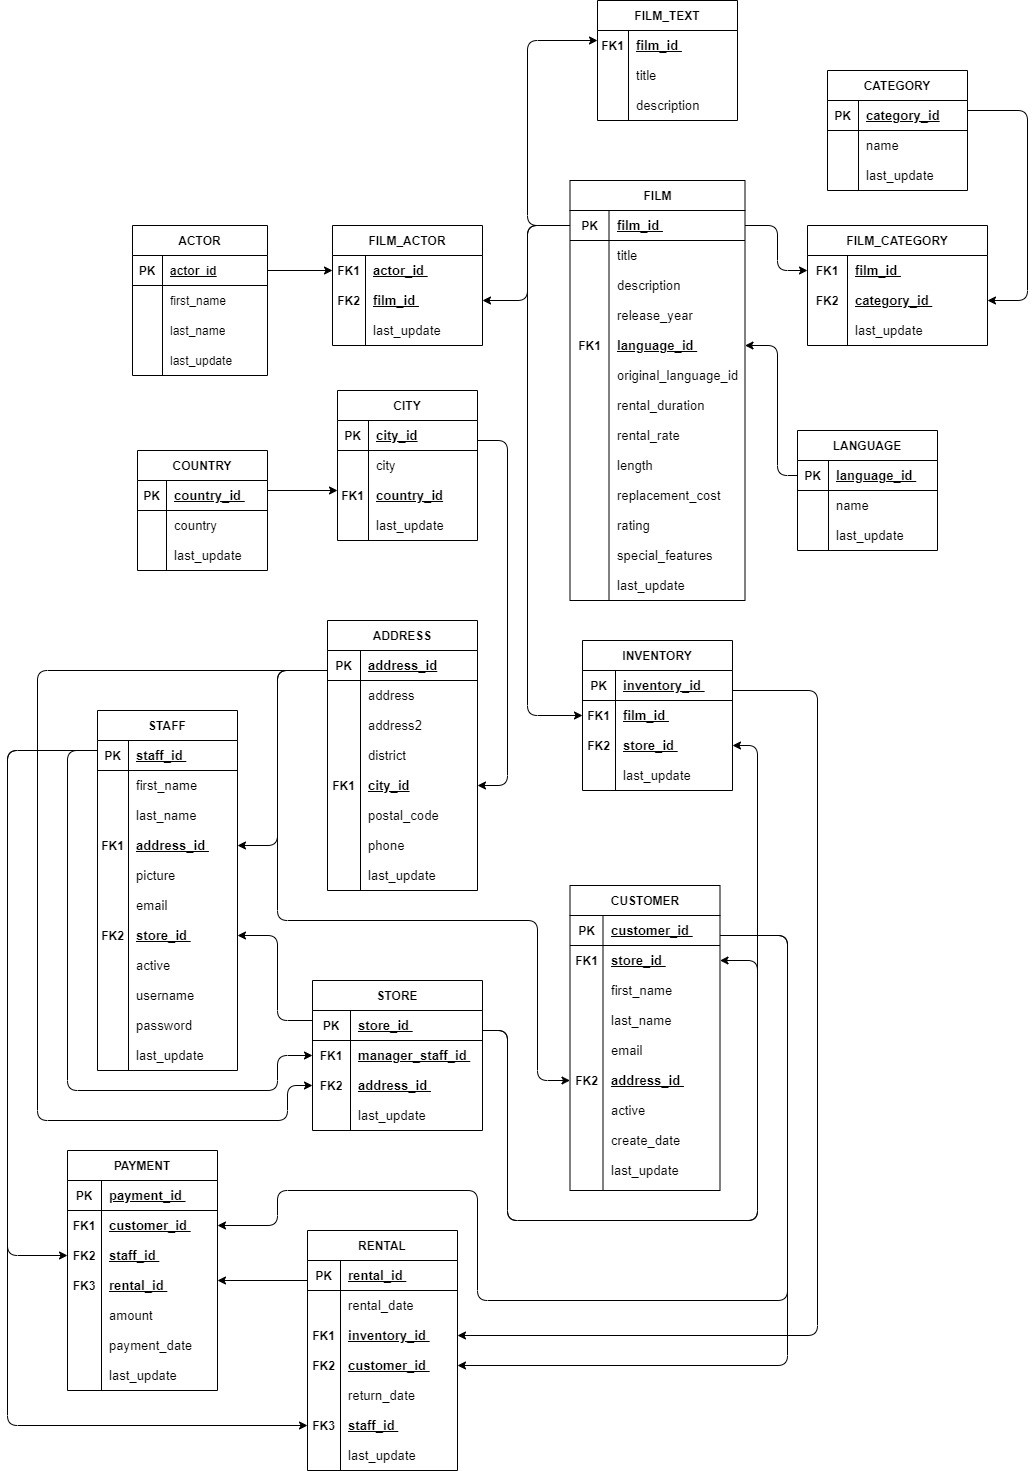
\includegraphics[width=\textwidth,height=15cm]{er_diagram}
		\caption{Proposed Entity Relation Diagram arrangement. \protect\footnotemark}	
	\end{figure}
	\footnotetext{This diagram is based on available table data provided.}


\subsection{Database Creation}
	\begin{figure}[H]
		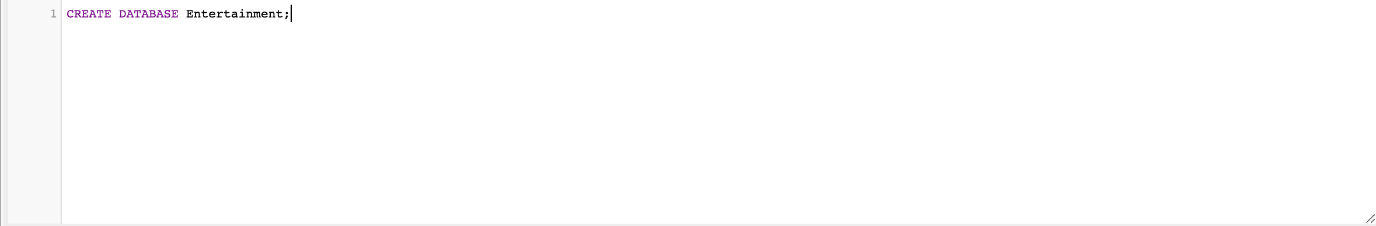
\includegraphics[width=\textwidth]{database_create}
		\caption{Creation of database "Entertainment"}	
	\end{figure}
	\rule{\textwidth}{0.4pt}
\subsection{Creation and Insertion of Tables}
	\begin{figure}[H]
		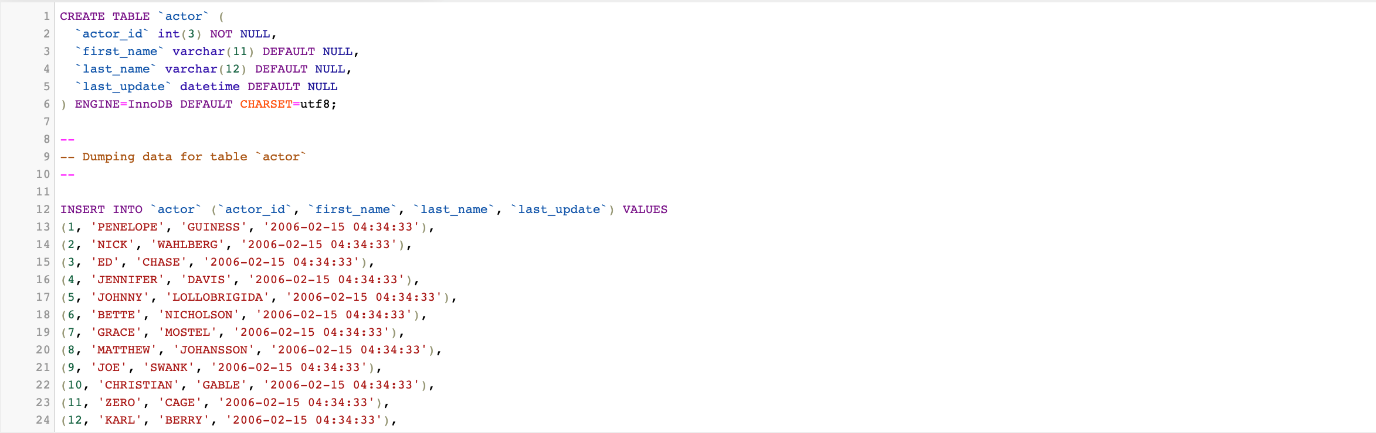
\includegraphics[width=\textwidth]{table_actor_cins}
		\caption{Creation and Insertion of table "Actor"}	
	\end{figure}
	\begin{figure}[H]
		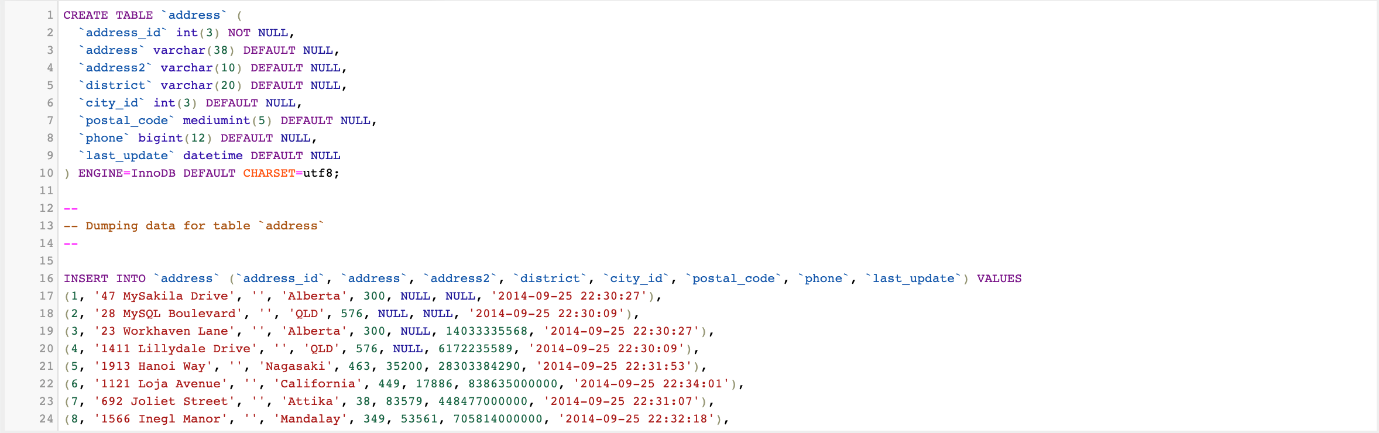
\includegraphics[width=\textwidth]{table_address_cins}
		\caption{Creation and Insertion of table "Address"}	
	\end{figure}
	\begin{figure}[H]
		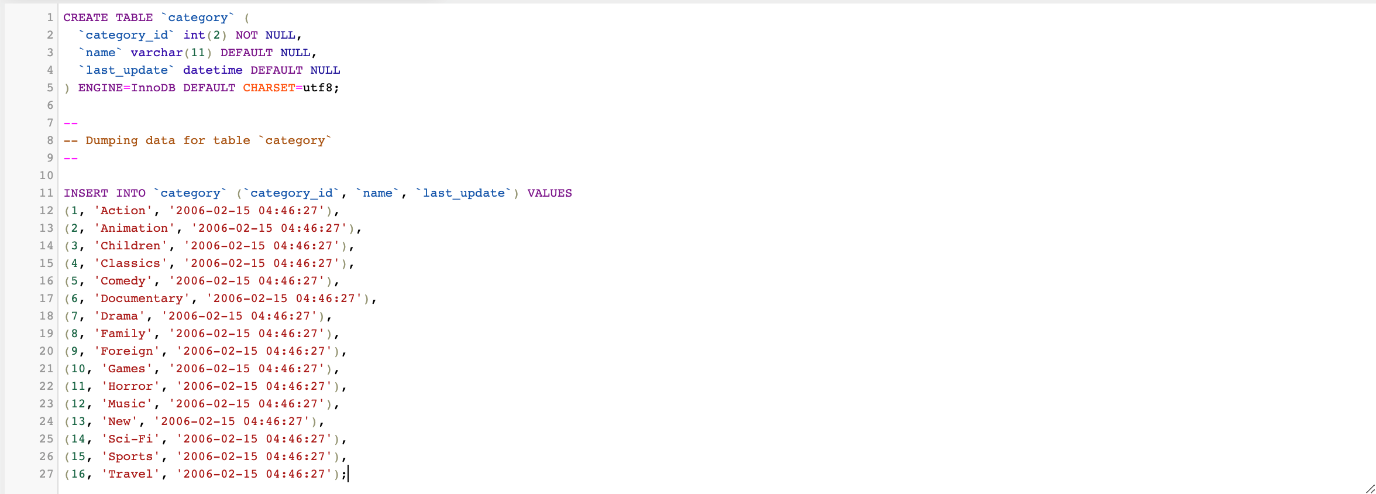
\includegraphics[width=\textwidth]{table_category_cins}
		\caption{Creation and Insertion of table "Category"}	
	\end{figure}
	\begin{figure}[H]
		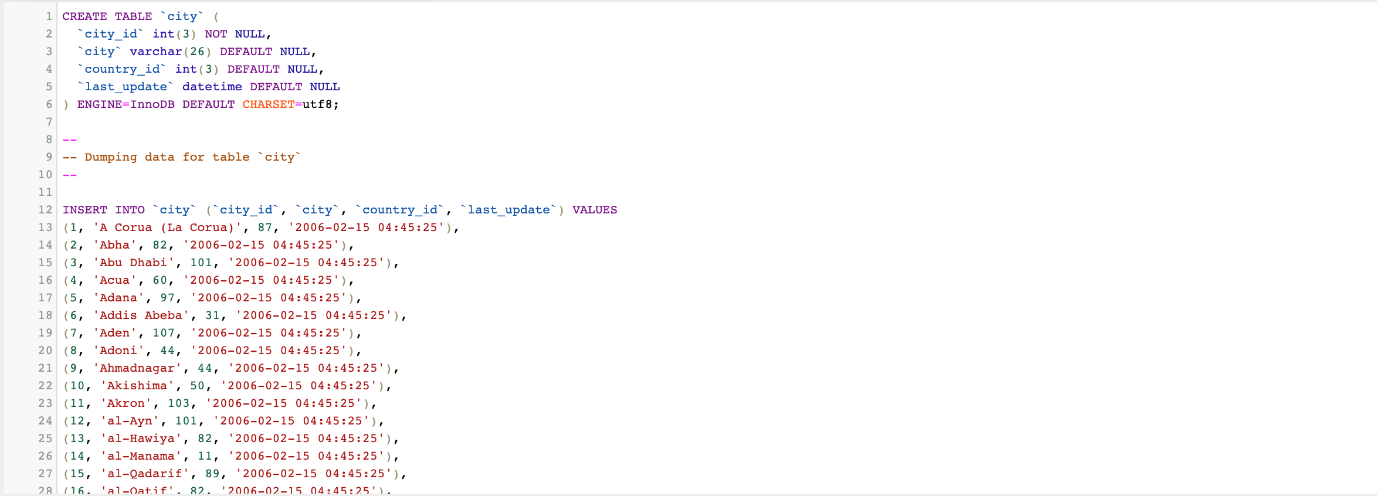
\includegraphics[width=\textwidth]{table_city_cins}
		\caption{Creation and Insertion of table "City"}	
	\end{figure}
	\begin{figure}[H]
		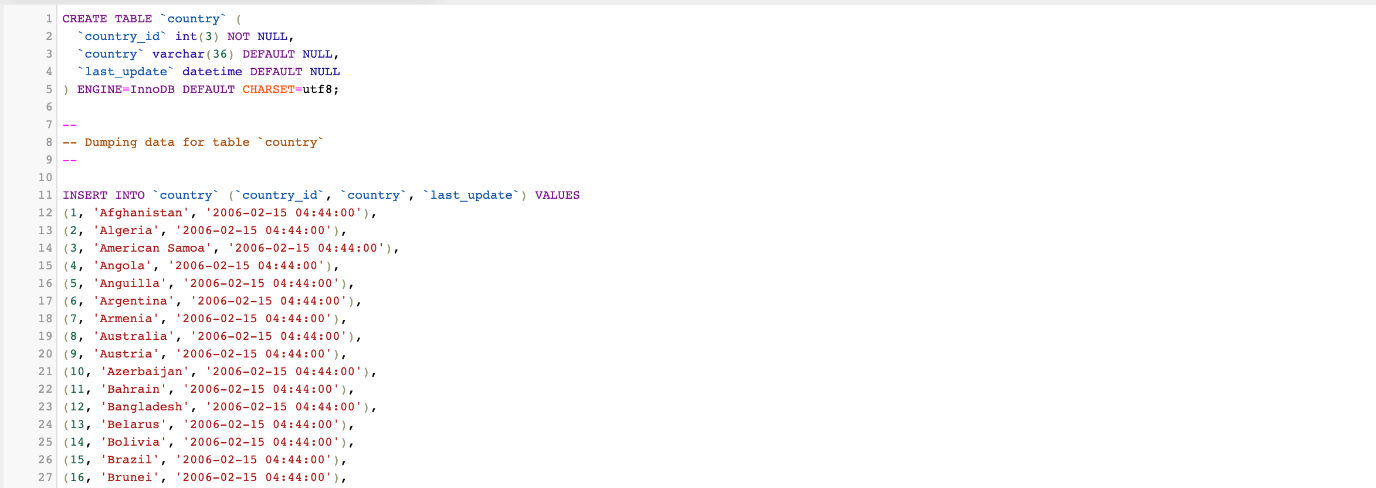
\includegraphics[width=\textwidth]{table_country_cins}
		\caption{Creation and Insertion of table "Country"}	
	\end{figure}
	\begin{figure}[H]
		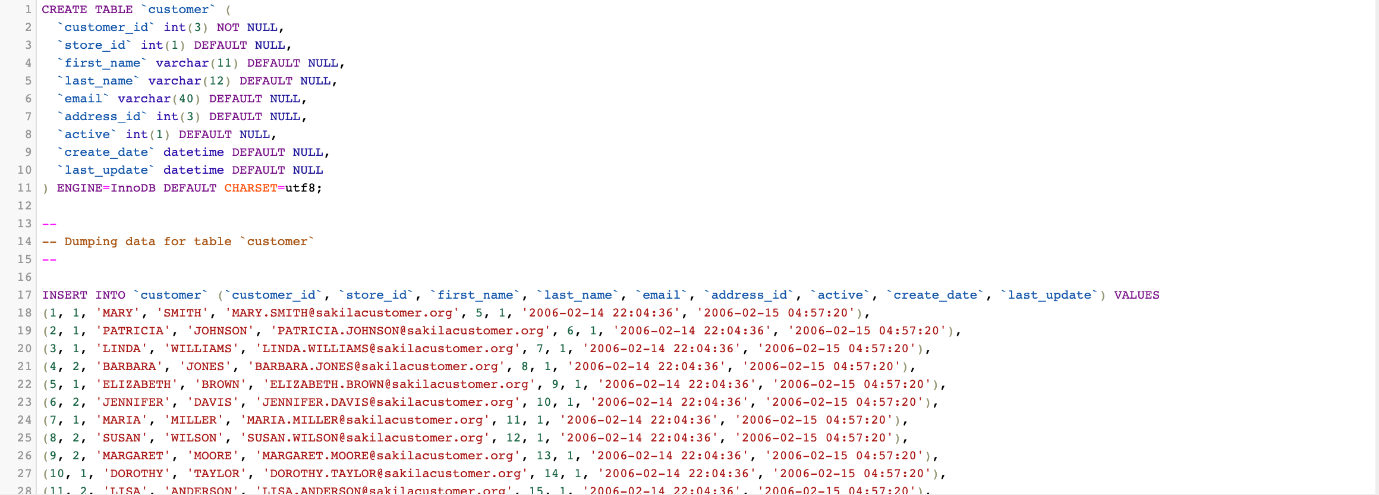
\includegraphics[width=\textwidth]{table_customer_cins}
		\caption{Creation and Insertion of table "Customer"}	
	\end{figure}
	Note that the original\textunderscore language\textunderscore id column's datatype is converted to an \textbf{int} later due to foreign key changes after normaliztion.
	\begin{figure}[H]
		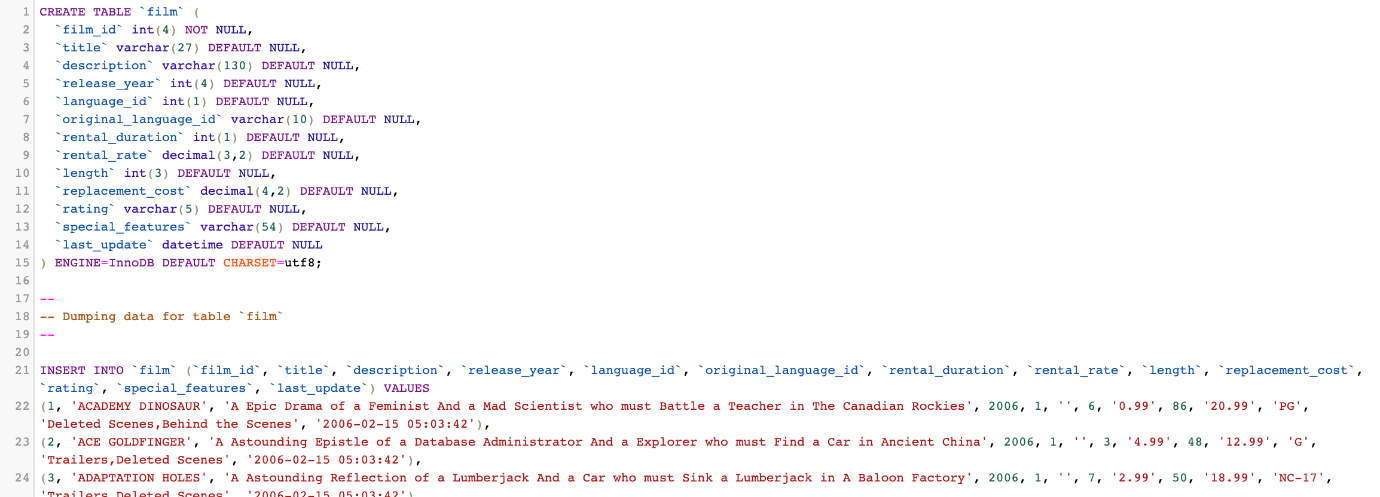
\includegraphics[width=\textwidth]{table_film_cins}
		\caption{Creation and Insertion of table "Film"}	
	\end{figure}
	\begin{figure}[H]
		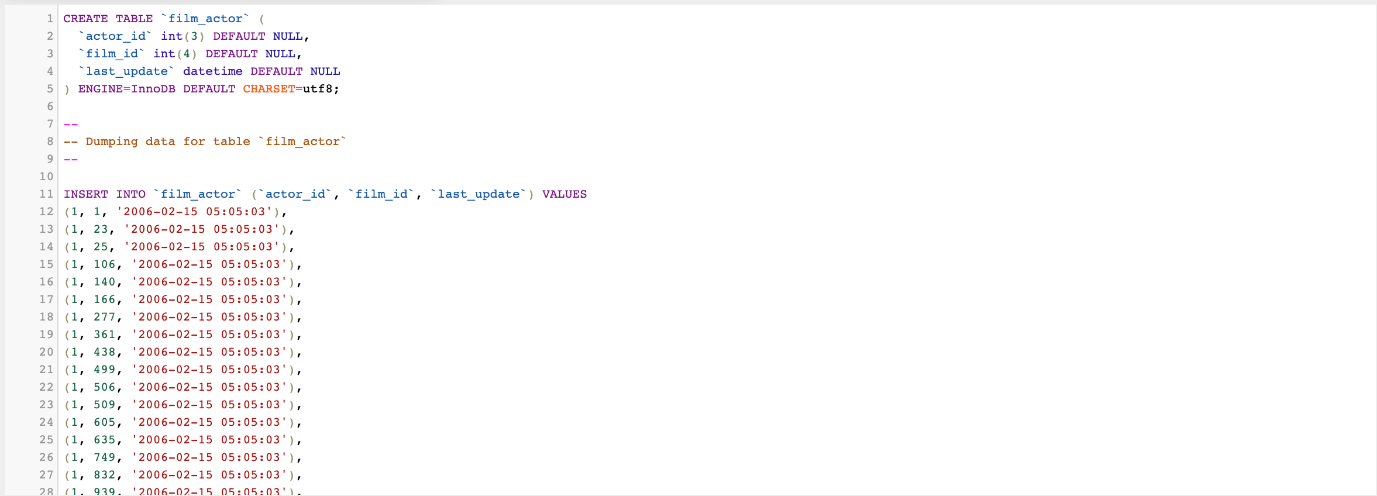
\includegraphics[width=\textwidth]{table_filmactor_cins}
		\caption{Creation and Insertion of table "Film\textunderscore Actor"}	
	\end{figure}
	\begin{figure}[H]
		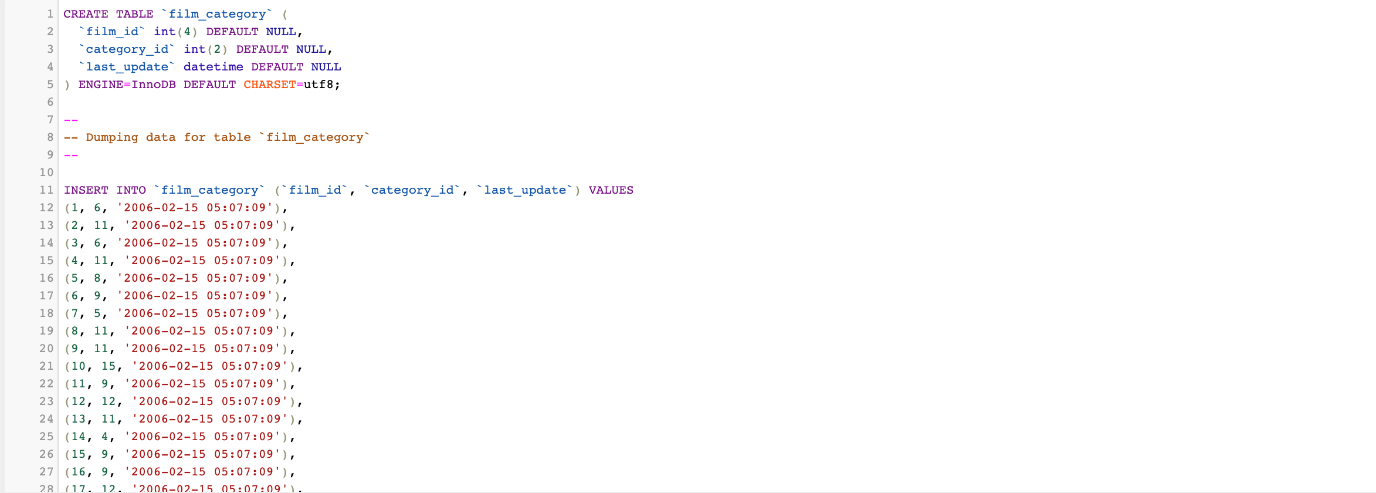
\includegraphics[width=\textwidth]{table_filmcategory_cins}
		\caption{Creation and Insertion of table "Film\textunderscore Category"}	
	\end{figure}
	\begin{figure}[H]
		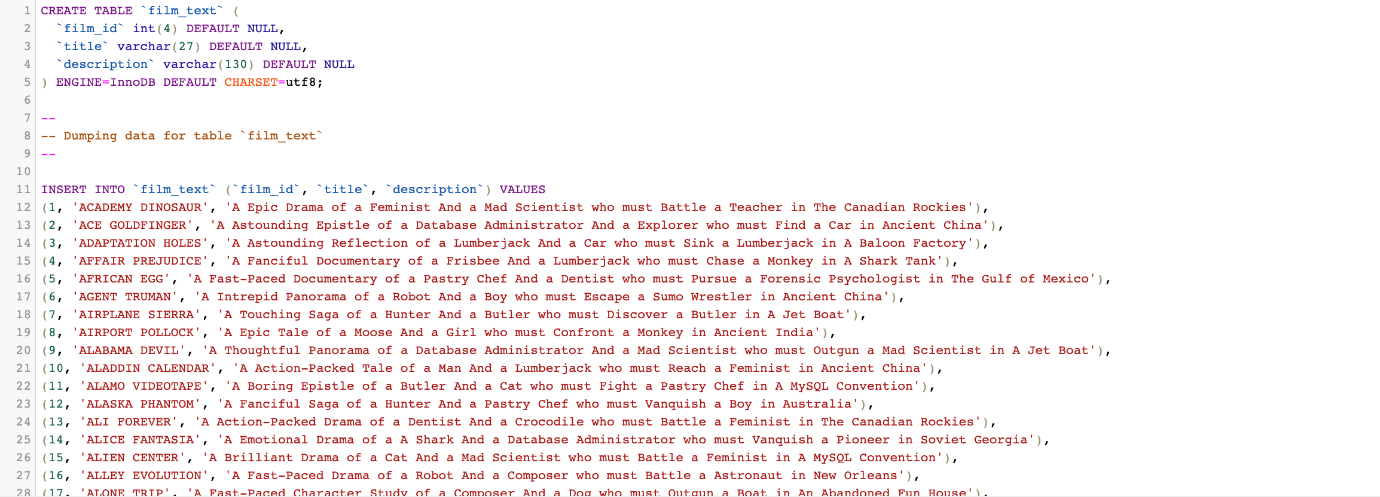
\includegraphics[width=\textwidth]{table_filmtext_cins}
		\caption{Creation and Insertion of table "Film\textunderscore Text"}	
	\end{figure}
	\begin{figure}[H]
		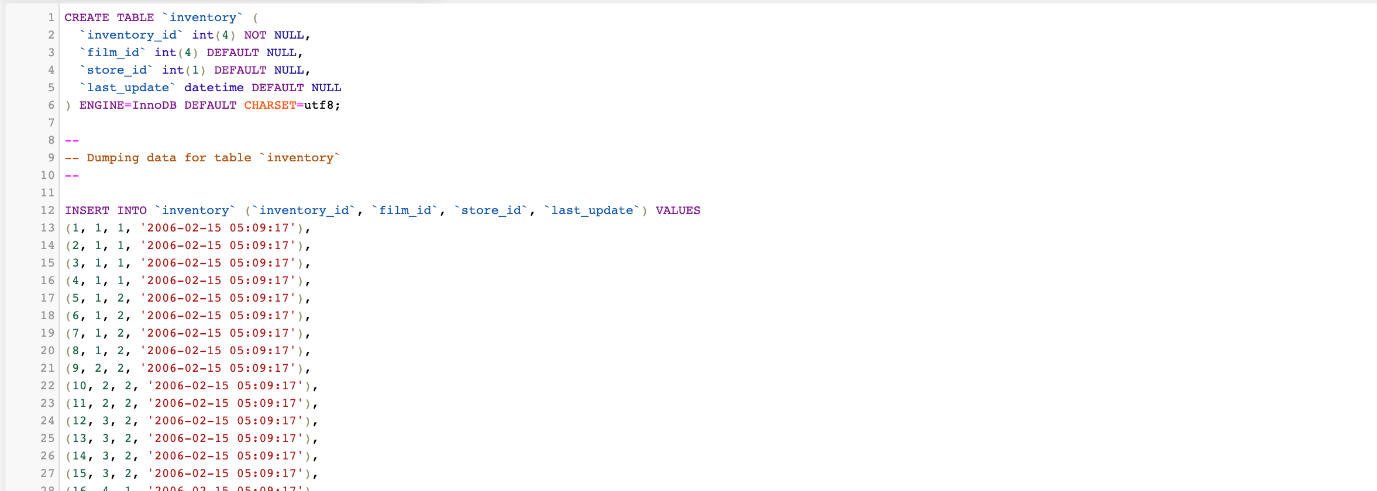
\includegraphics[width=\textwidth]{table_inventory_cins}
		\caption{Creation and Insertion of table "Inventory"}	
	\end{figure}
	\begin{figure}[H]
		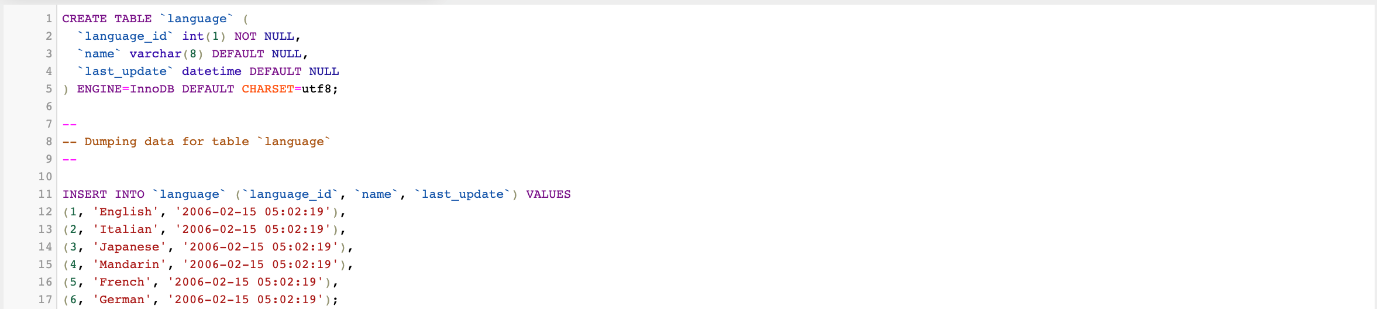
\includegraphics[width=\textwidth]{table_language_cins}
		\caption{Creation and Insertion of table "Language"}	
	\end{figure}
	\begin{figure}[H]
		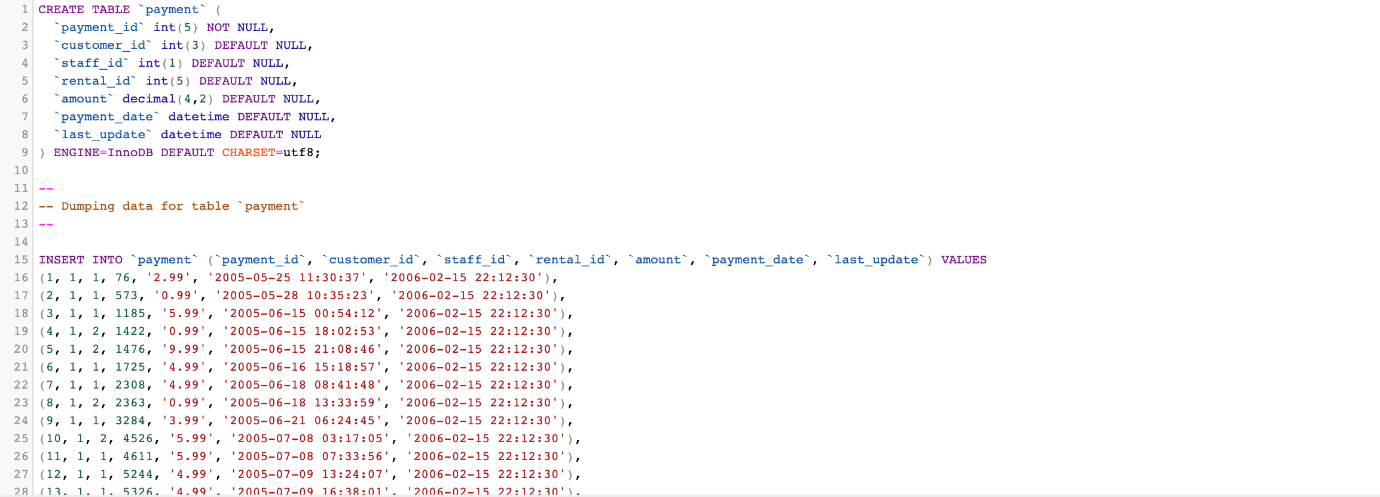
\includegraphics[width=\textwidth]{table_payment_cins}
		\caption{Creation and Insertion of table "Payment"}	
	\end{figure}
	\begin{figure}[H]
		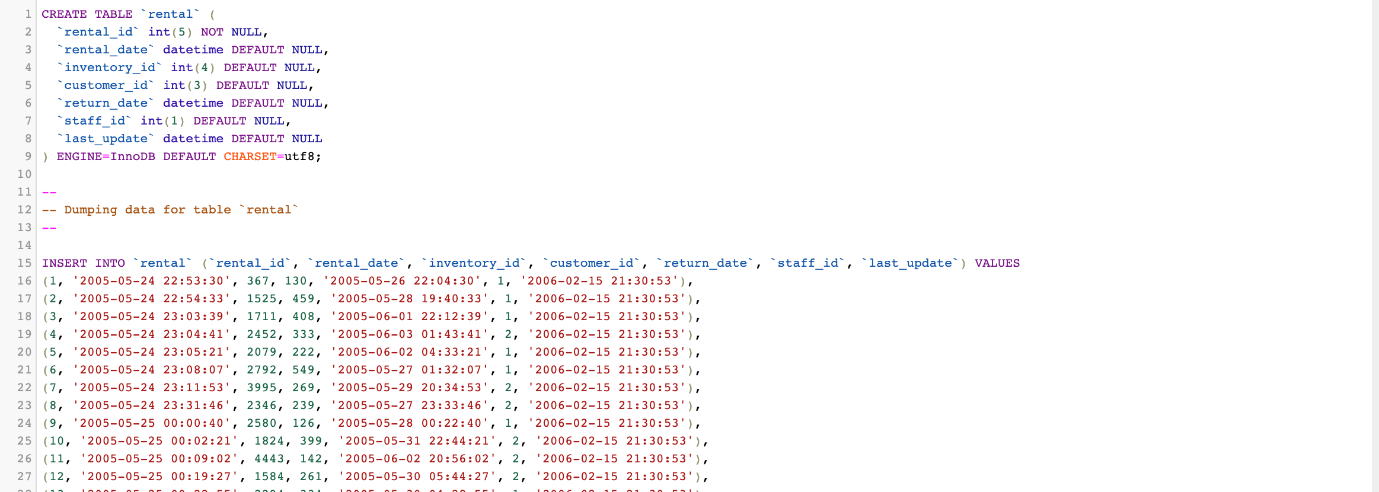
\includegraphics[width=\textwidth]{table_rental_cins}
		\caption{Creation and Insertion of table "Rental"}	
	\end{figure}
	\begin{figure}[H]
		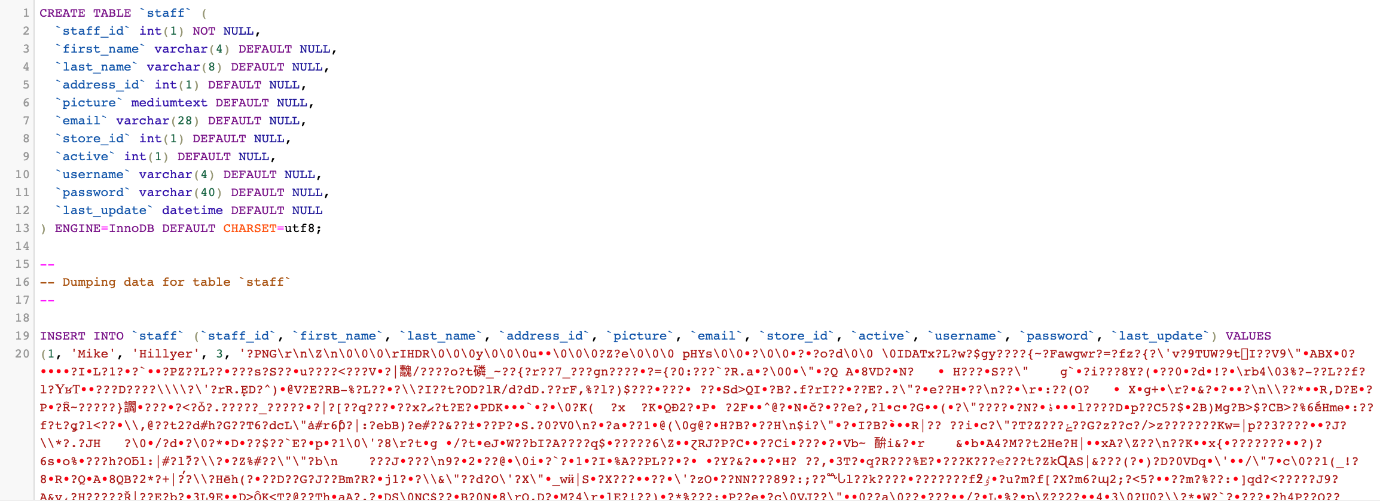
\includegraphics[width=\textwidth]{table_staff_cins}
		\caption{Creation and Insertion of table "Staff"}	
	\end{figure}
	\begin{figure}[H]
		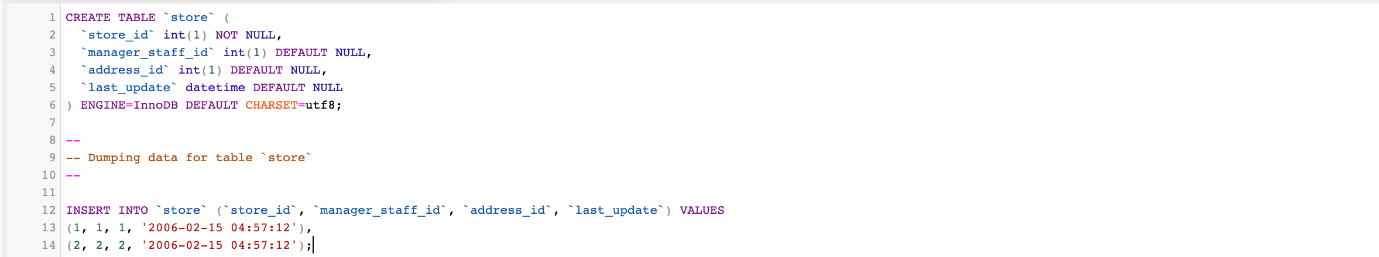
\includegraphics[width=\textwidth]{table_store_cins}
		\caption{Creation and Insertion of table "Store"}	
	\end{figure}

\subsection{Table Constraints (Foreign Keys)}
	\begin{figure}[H]
		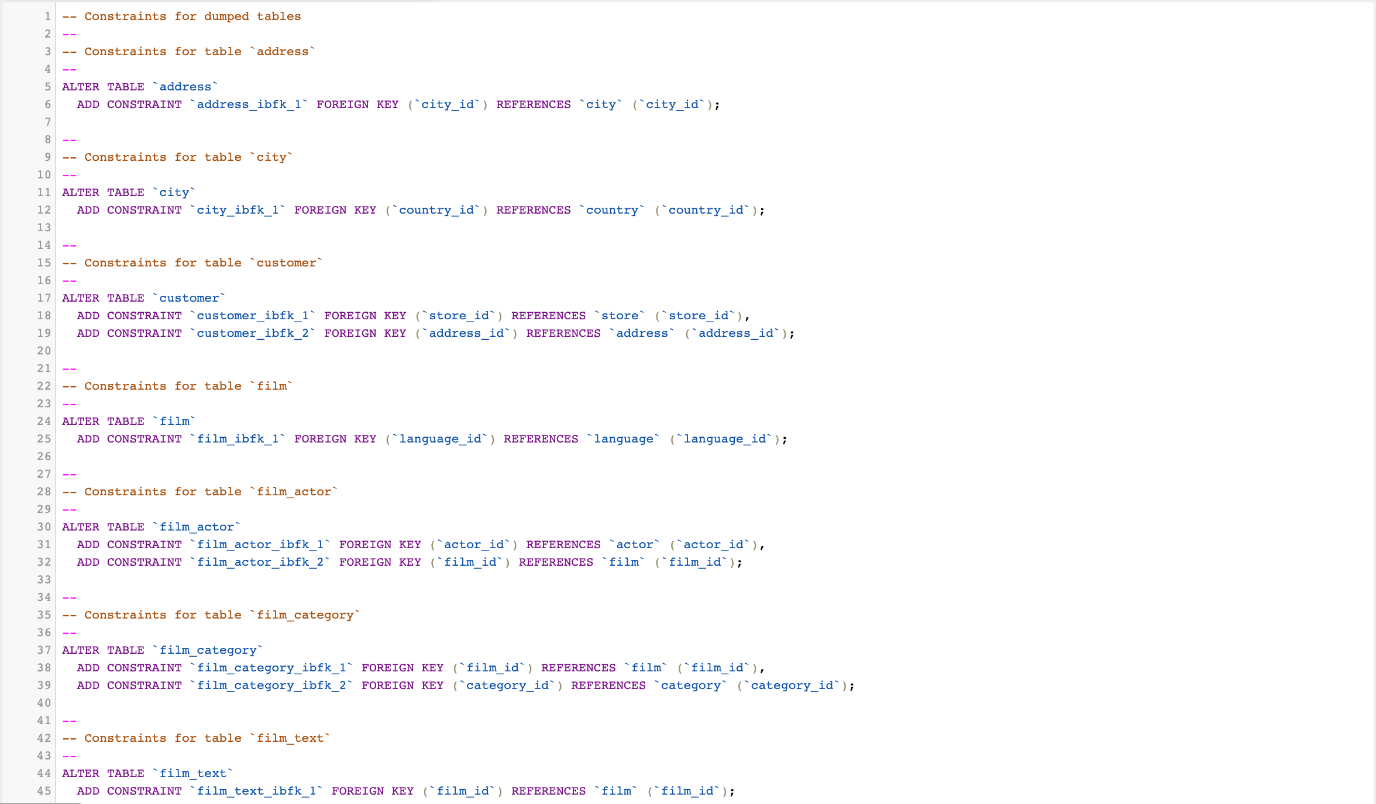
\includegraphics[width=\textwidth]{tableconstraints1}
		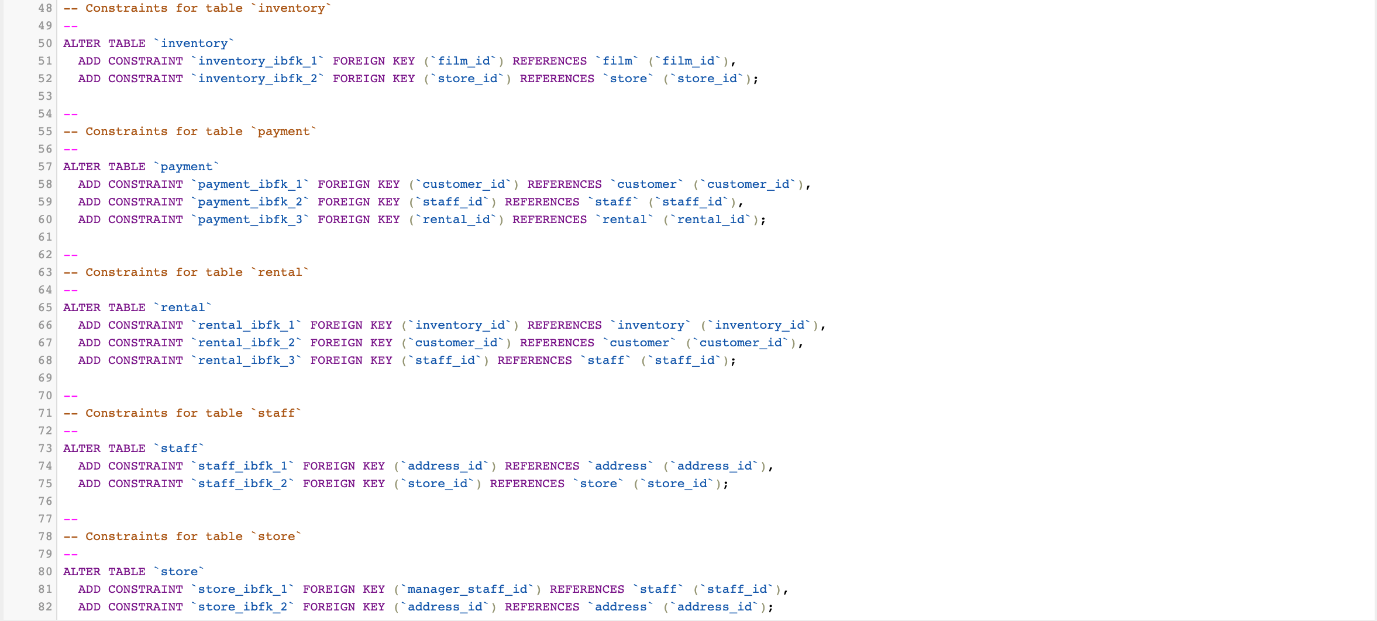
\includegraphics[width=\textwidth]{tableconstraints2}
	\end{figure}

\subsection{Table Indexes (Primary/Foreign Keys)}
	Amendment: original\textunderscore language\textunderscore id in the "Film" table is later linked to the "Language" table as a foreign key in the current database version after normalization.
	\begin{figure}[H]
		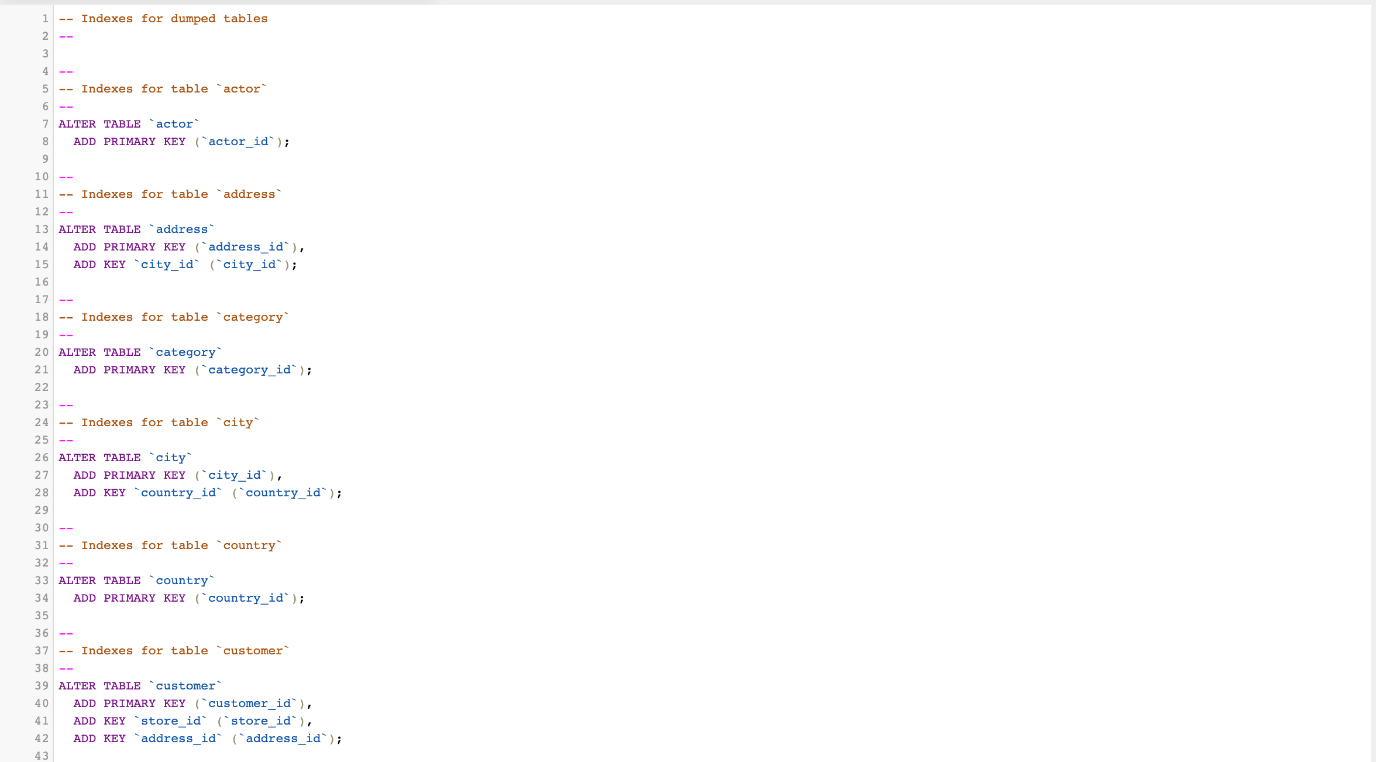
\includegraphics[width=\textwidth]{tableindexkeys1}
		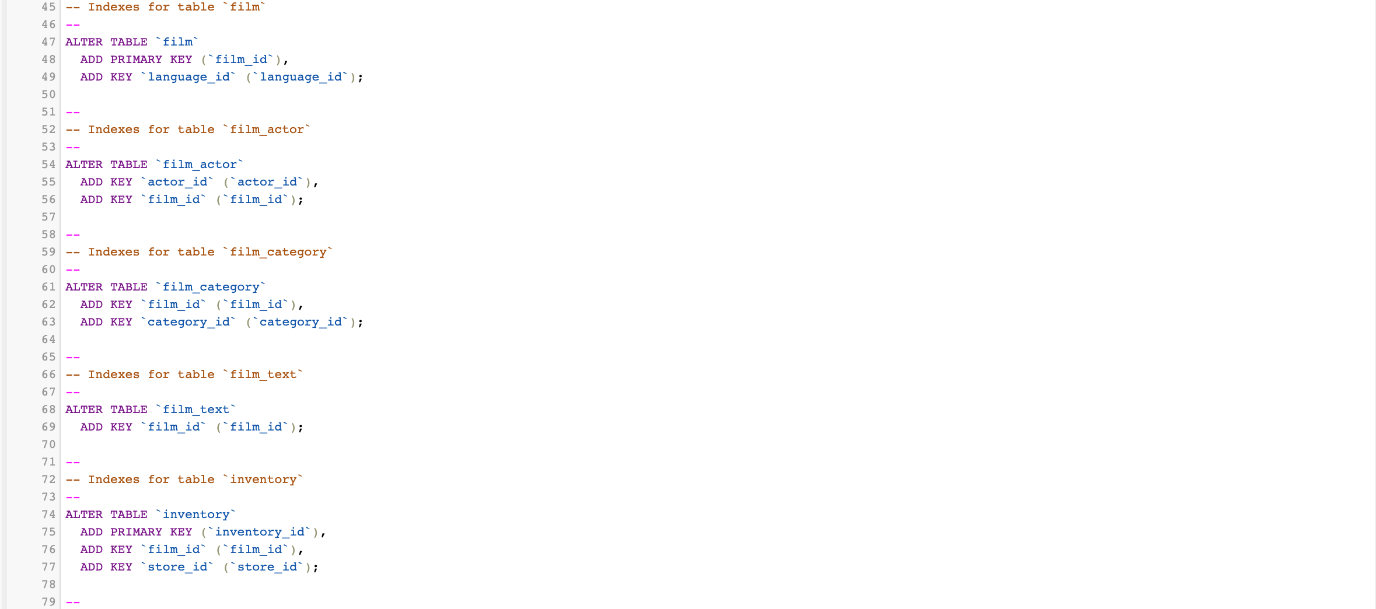
\includegraphics[width=\textwidth]{tableindexkeys2}
		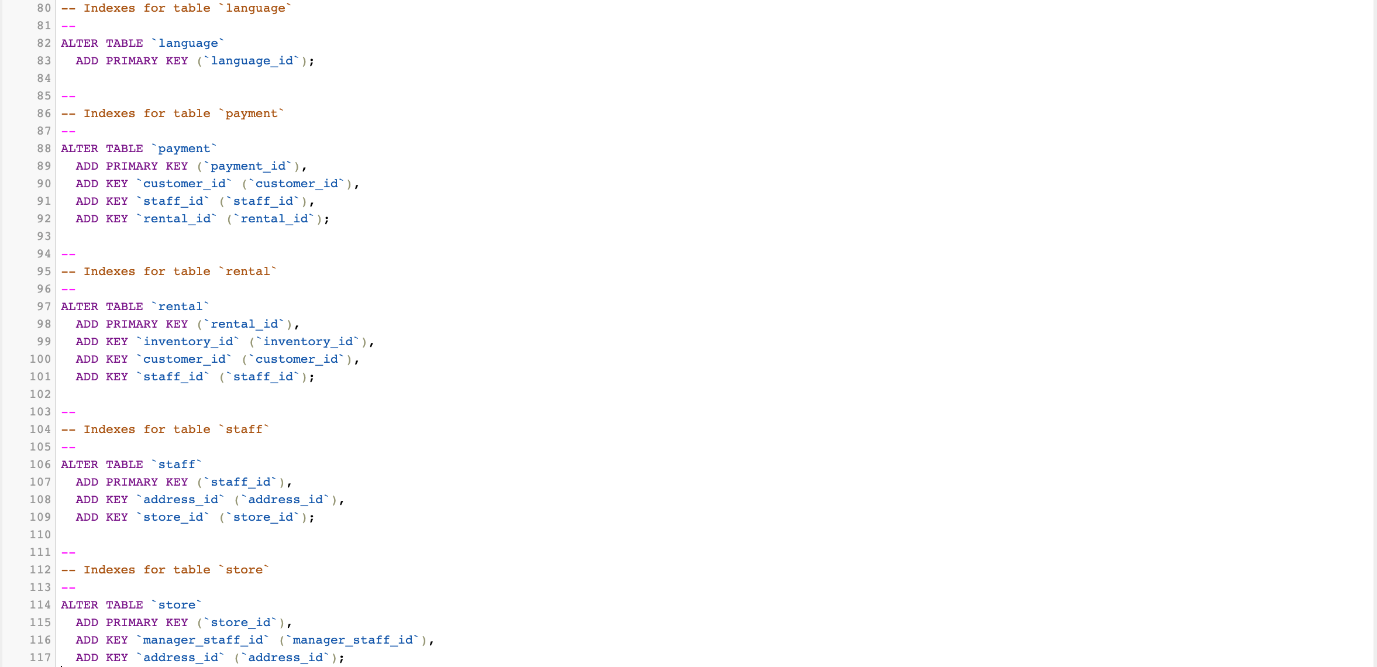
\includegraphics[width=\textwidth]{tableindexkeys3}
	\end{figure}	

\subsection{Table Structures}
	\begin{figure}[H]
		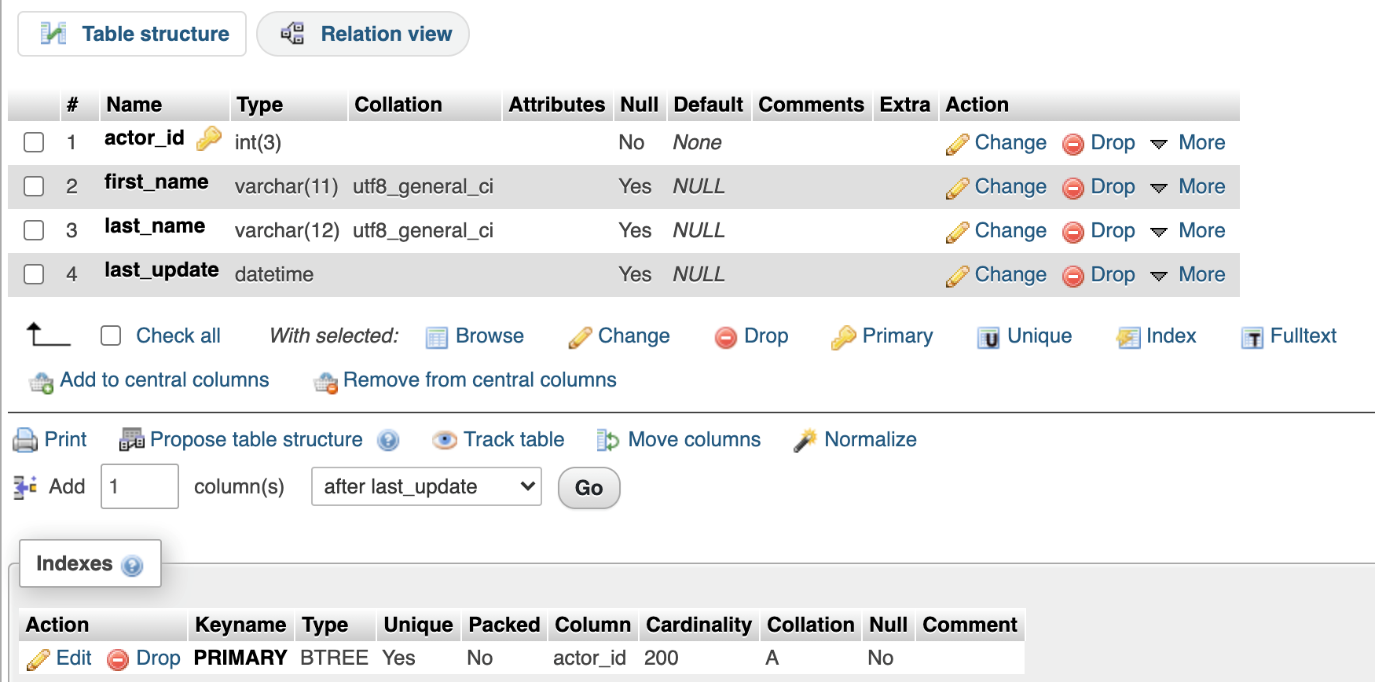
\includegraphics[width=\textwidth]{table_actor_struct}
		\caption{Structure of table "Actor"}	
	\end{figure}
	\begin{figure}[H]
		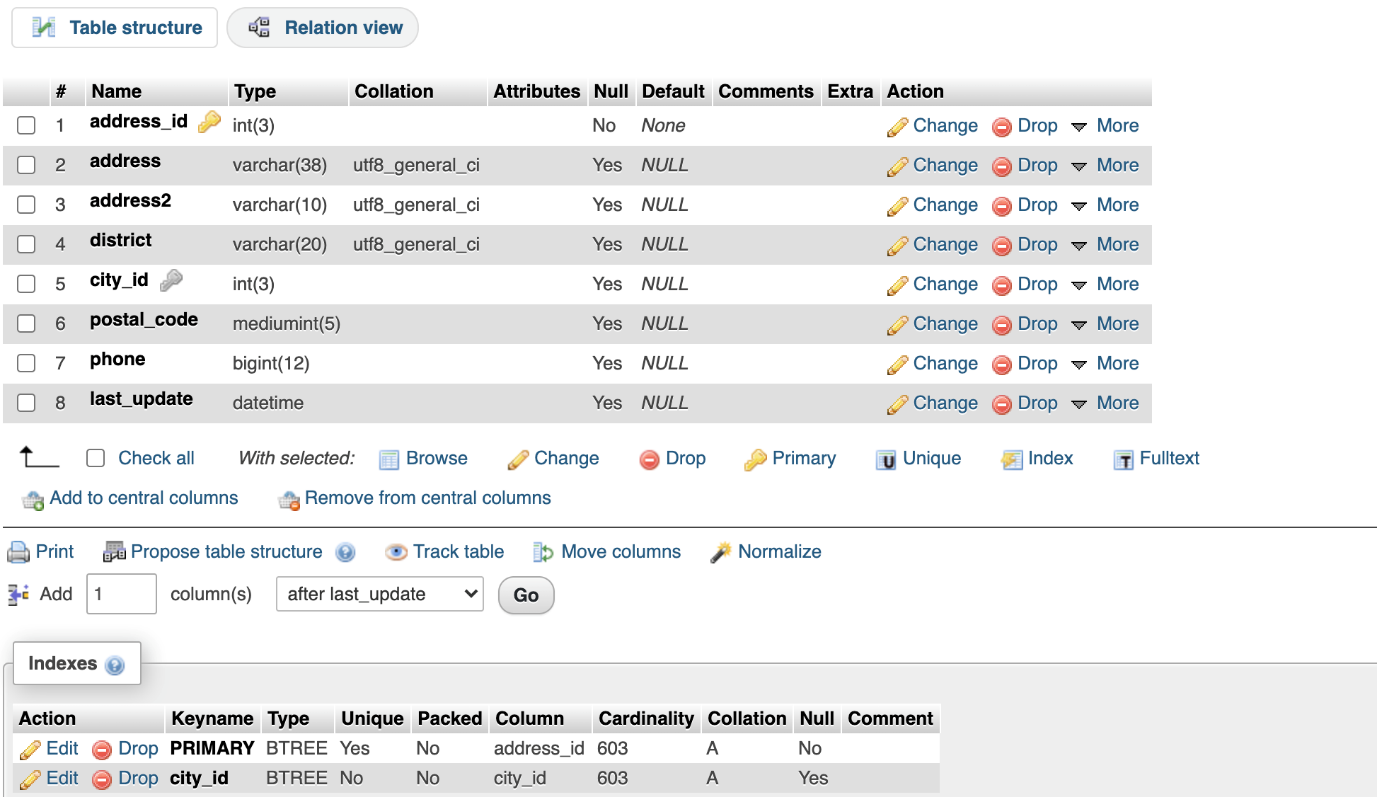
\includegraphics[width=\textwidth]{table_address_struct}
		\caption{Structure of table "Address"}	
	\end{figure}
	\begin{figure}[H]
		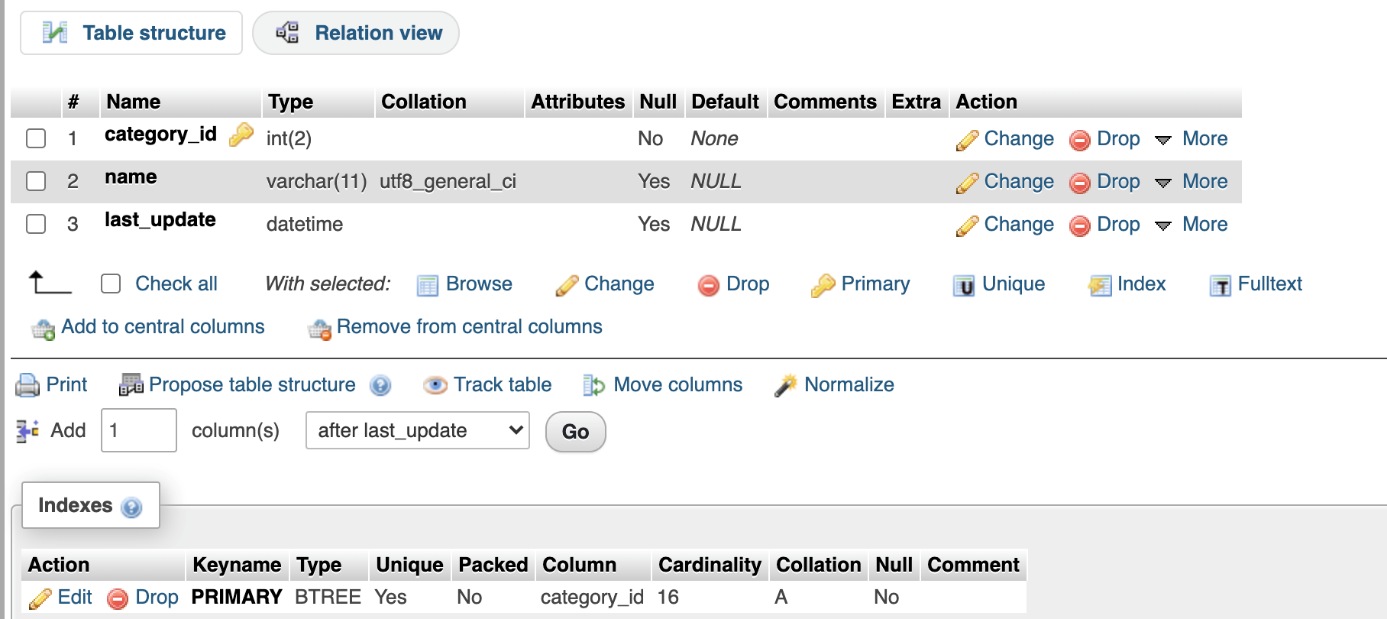
\includegraphics[width=\textwidth]{table_category_struct}
		\caption{Structure of table "Category"}	
	\end{figure}
	\begin{figure}[H]
		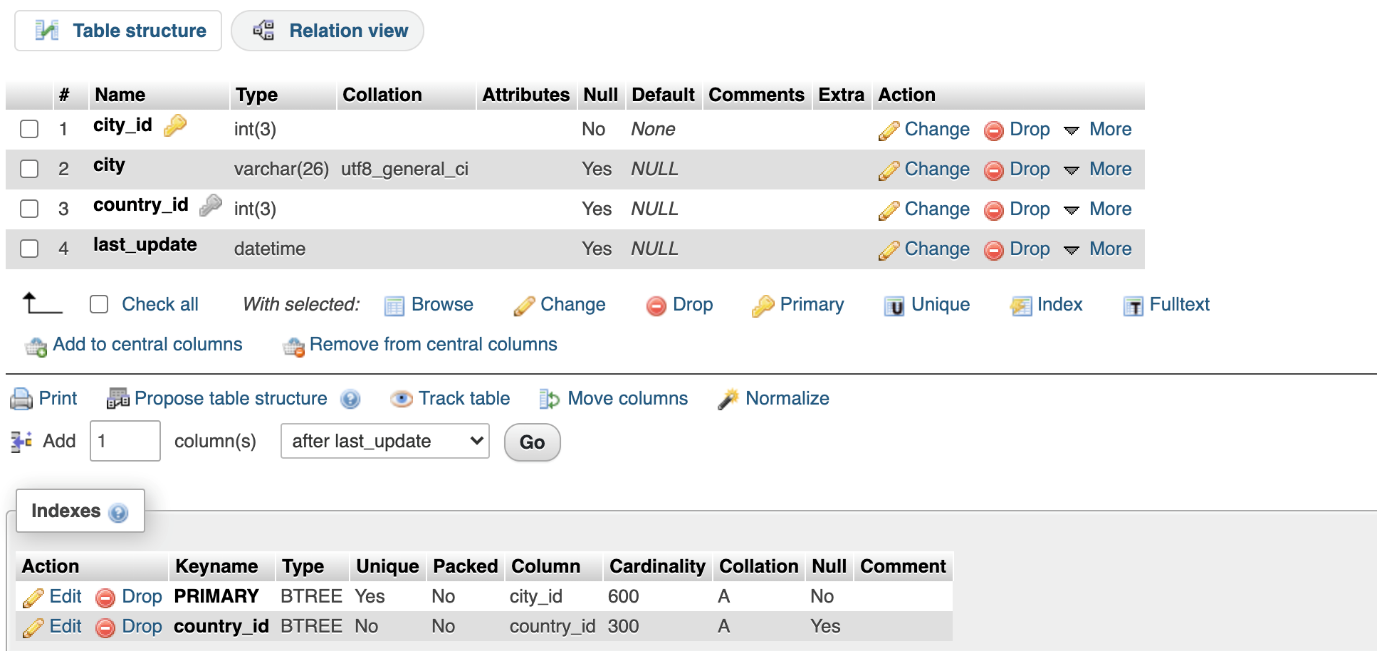
\includegraphics[width=\textwidth]{table_city_struct}
		\caption{Structure of table "City"}	
	\end{figure}
	\begin{figure}[H]
		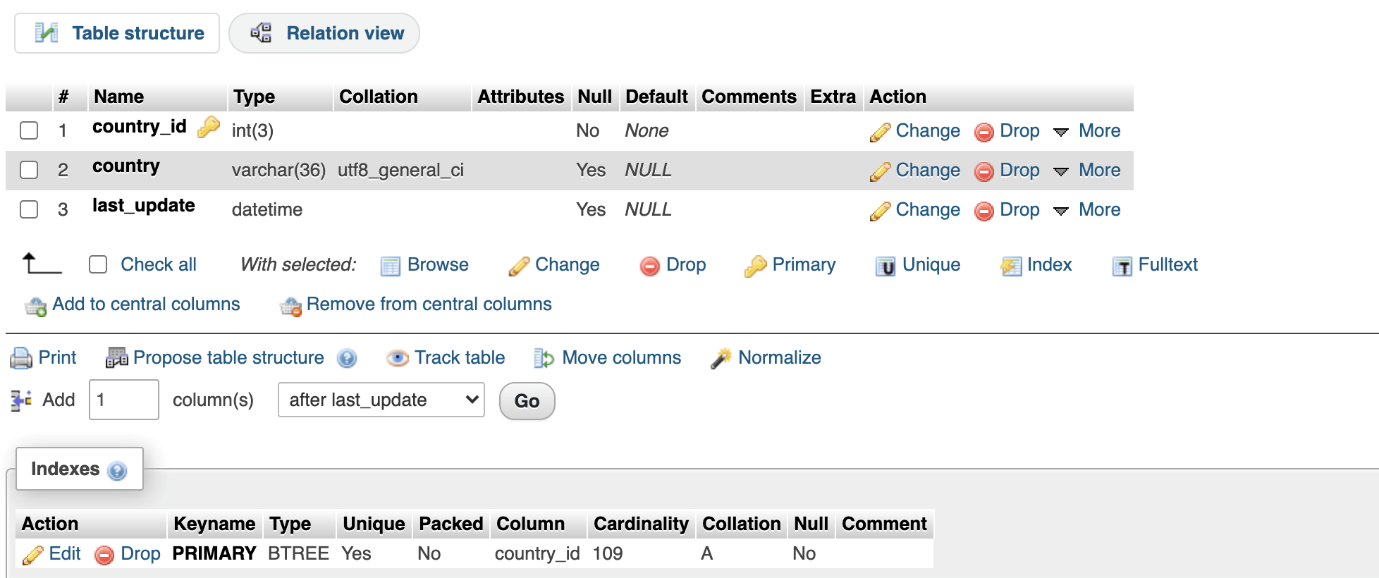
\includegraphics[width=\textwidth]{table_country_struct}
		\caption{Structure of table "Country"}	
	\end{figure}
	\begin{figure}[H]
		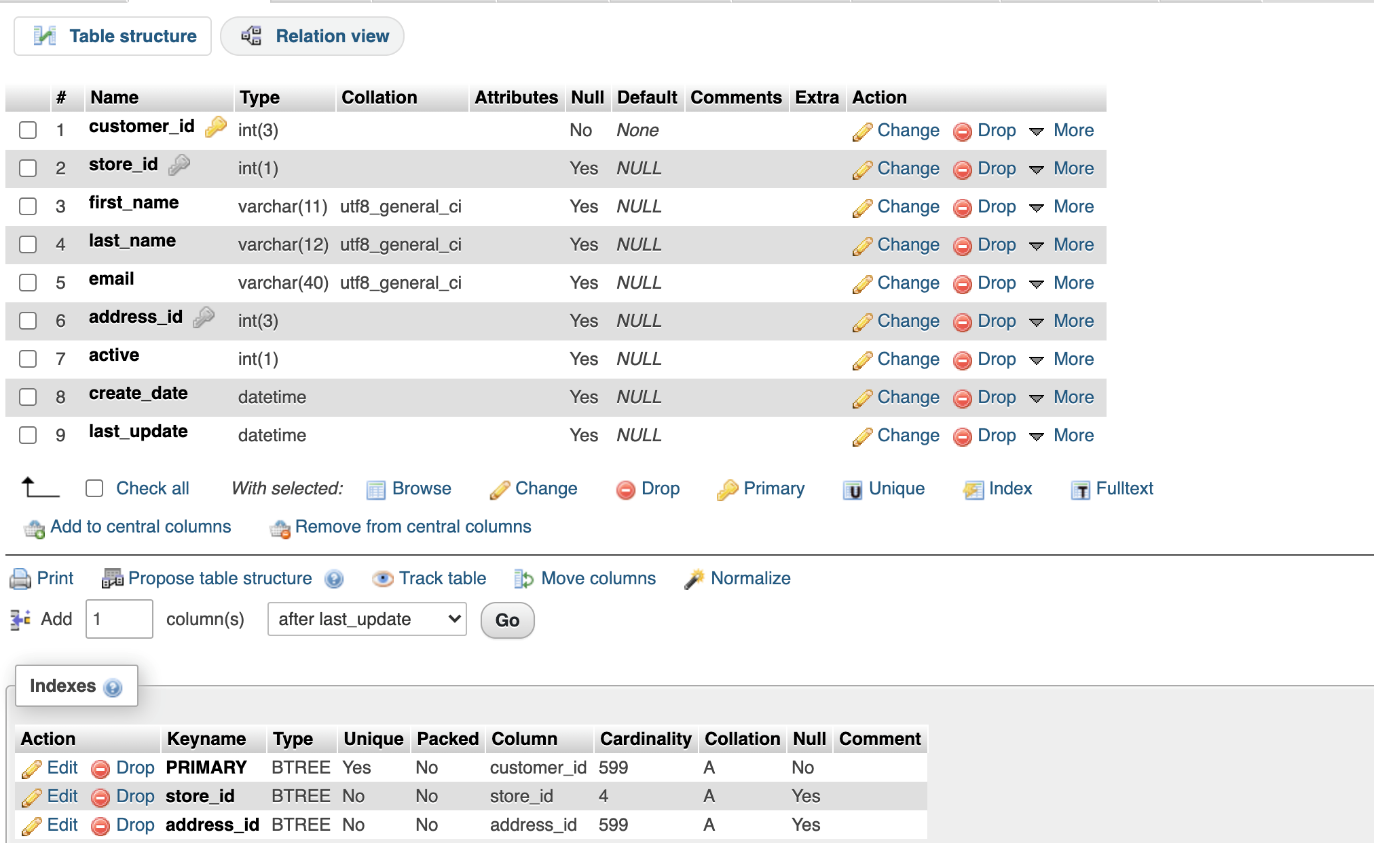
\includegraphics[width=\textwidth]{table_customer_struct}
		\caption{Structure of table "Customer"}	
	\end{figure}
	\begin{figure}[H]
		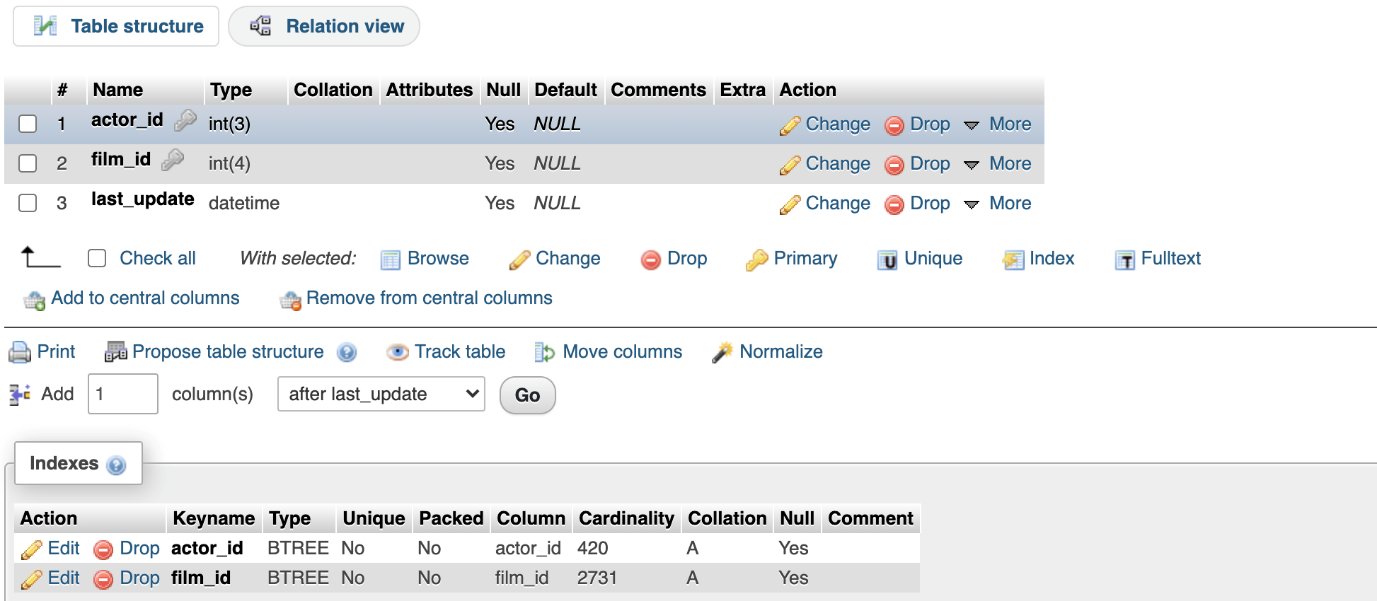
\includegraphics[width=\textwidth]{table_filmactor_struct}
		\caption{Structure of table "Film\textunderscore Actor"}	
	\end{figure}
	\begin{figure}[H]
		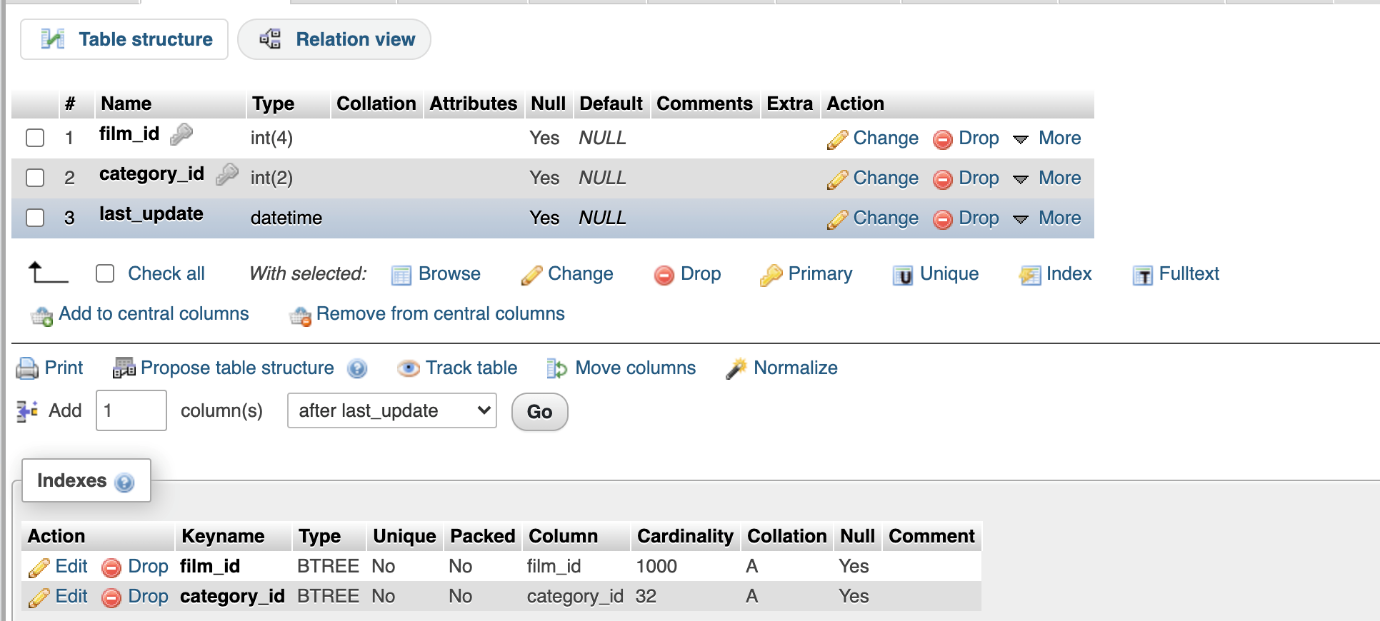
\includegraphics[width=\textwidth]{table_filmcategory_struct}
		\caption{Structure of table "Film\textunderscore Category"}	
	\end{figure}
	Amendment: The original\textunderscore language\textunderscore id field is represented as an \textbf{int} in the latest iteration of the database.
	\begin{figure}[H]
		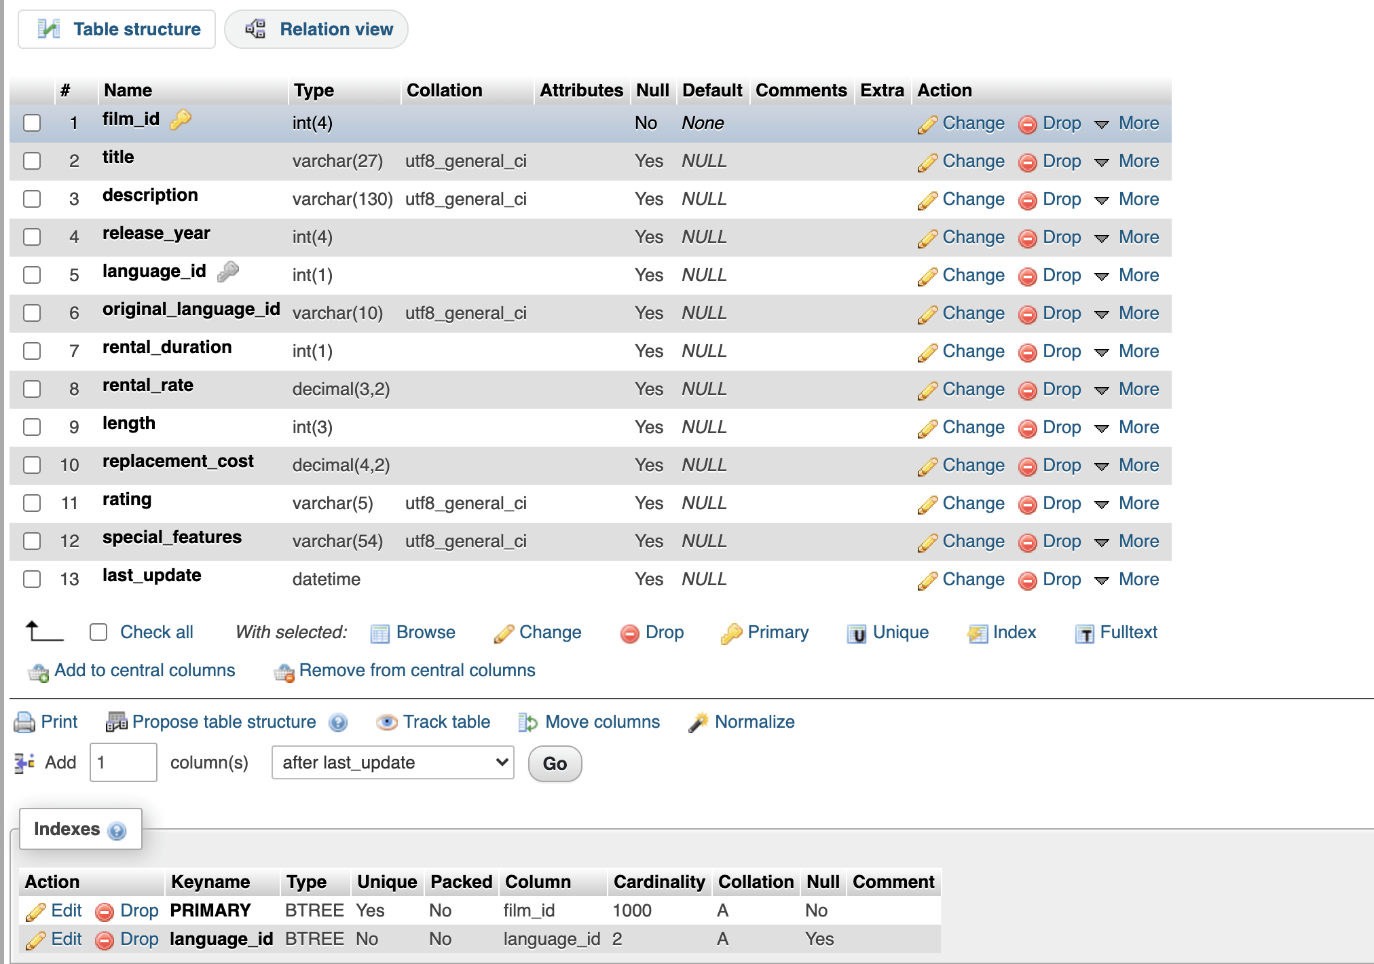
\includegraphics[width=\textwidth]{table_film_struct}
		\caption{Structure of table "Film"}	
	\end{figure}
	\begin{figure}[H]
		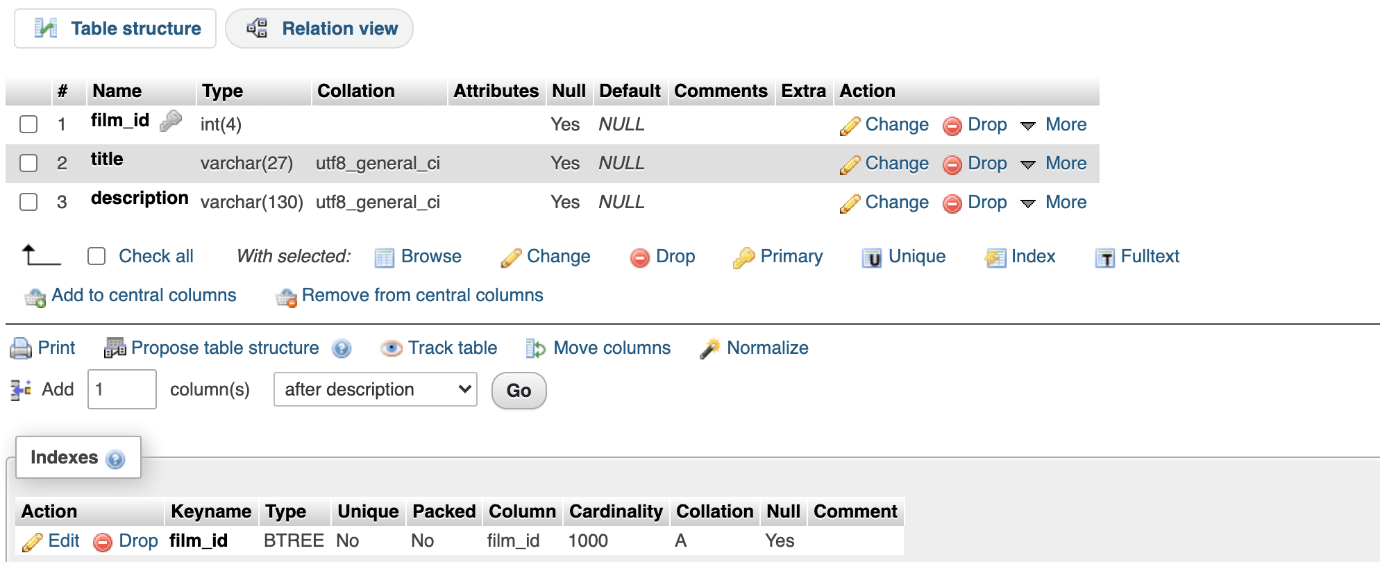
\includegraphics[width=\textwidth]{table_filmtext_struct}
		\caption{Structure of table "Film\textunderscore Text"}	
	\end{figure}
	\begin{figure}[H]
		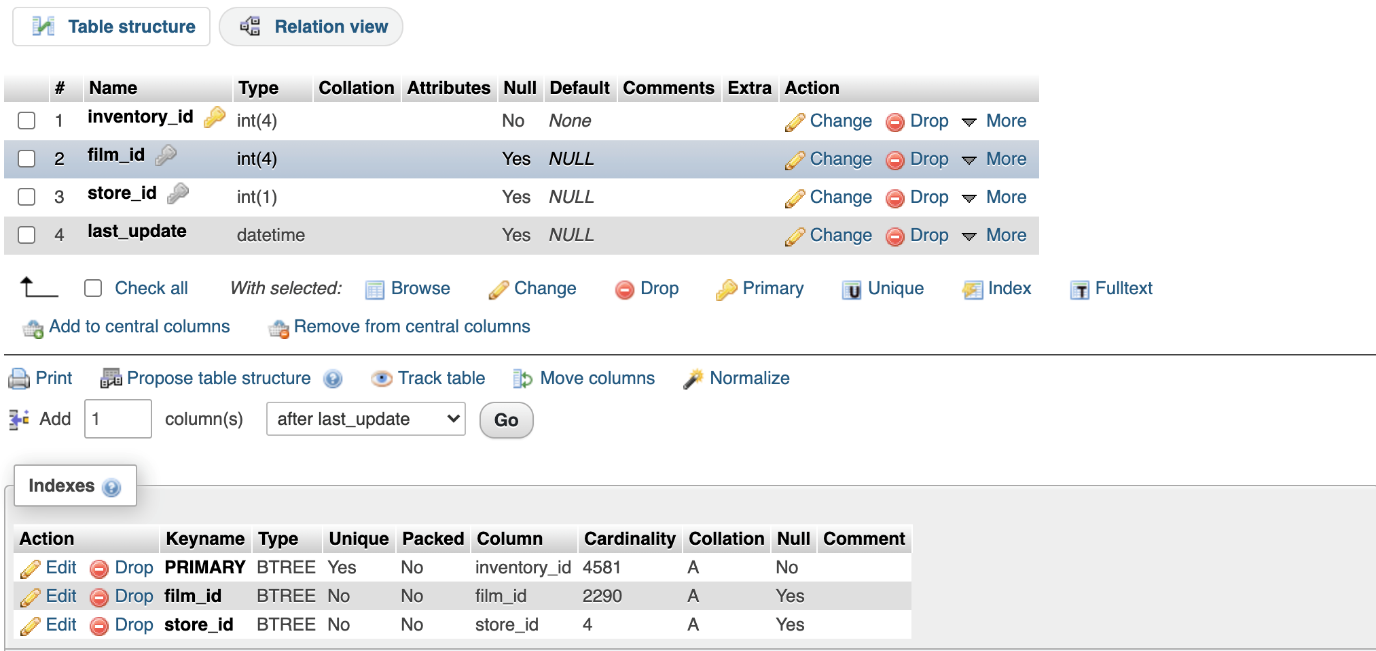
\includegraphics[width=\textwidth]{table_inventory_struct}
		\caption{Structure of table "Inventory"}	
	\end{figure}
	\begin{figure}[H]
		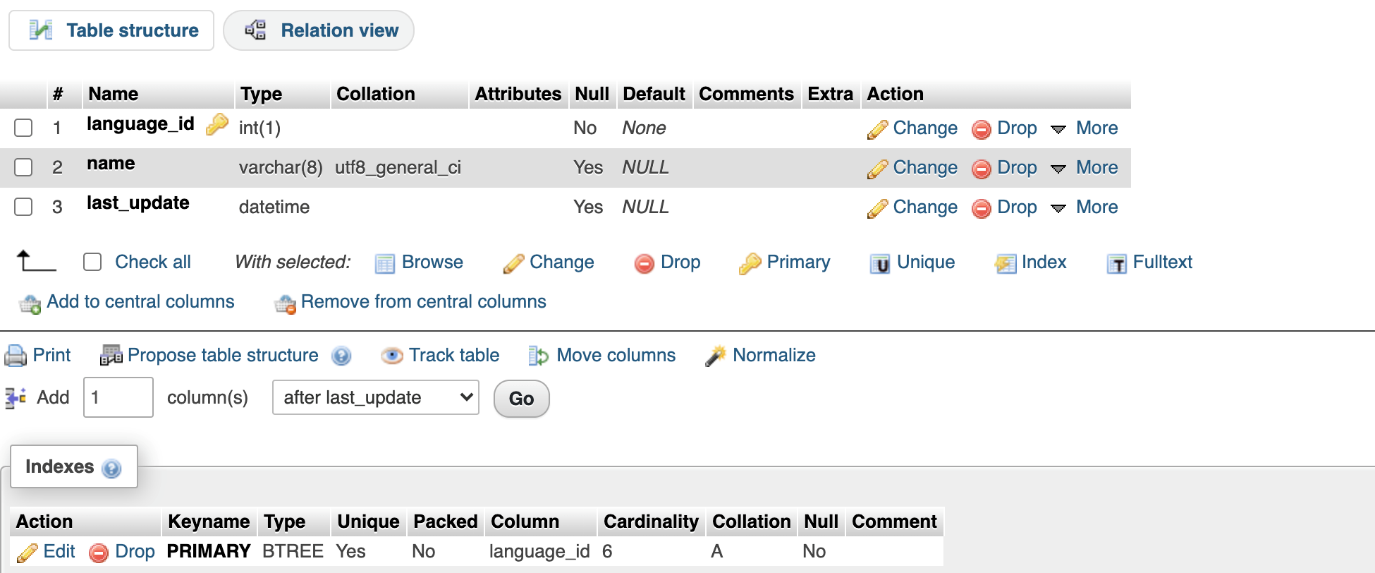
\includegraphics[width=\textwidth]{table_language_struct}
		\caption{Structure of table "Language"}	
	\end{figure}
	\begin{figure}[H]
		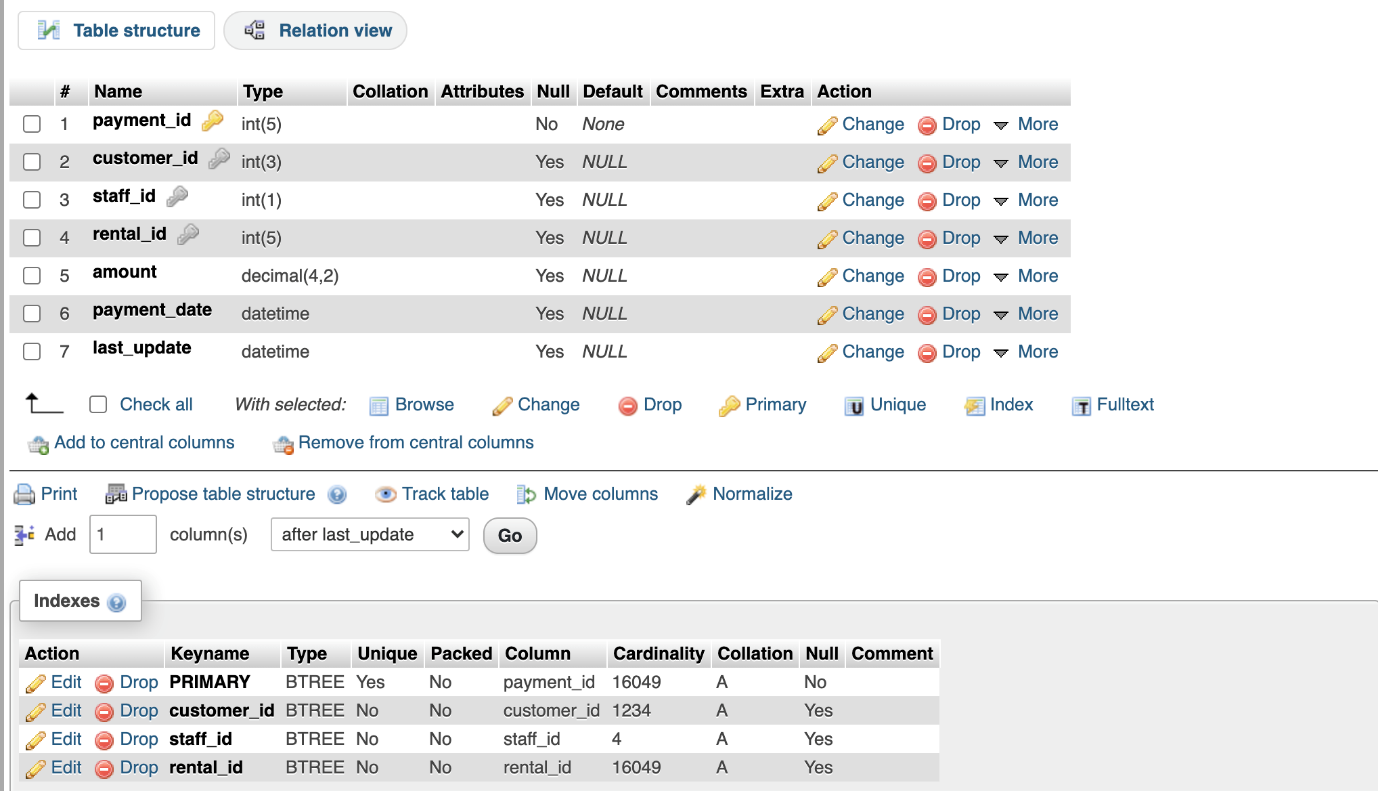
\includegraphics[width=\textwidth]{table_payment_struct}
		\caption{Structure of table "Payment"}	
	\end{figure}
	\begin{figure}[H]
		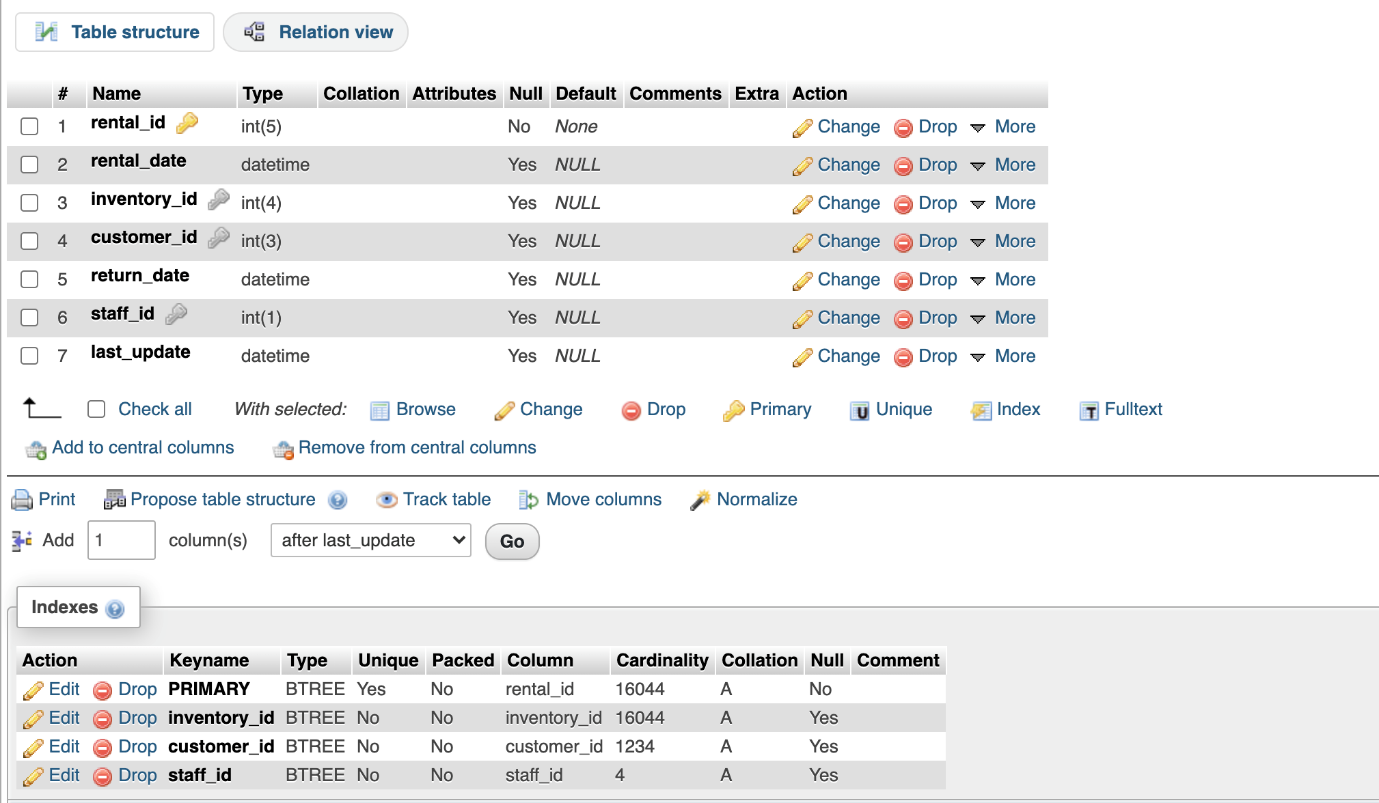
\includegraphics[width=\textwidth]{table_rental_struct}
		\caption{Structure of table "Rental"}	
	\end{figure}
	\begin{figure}[H]
		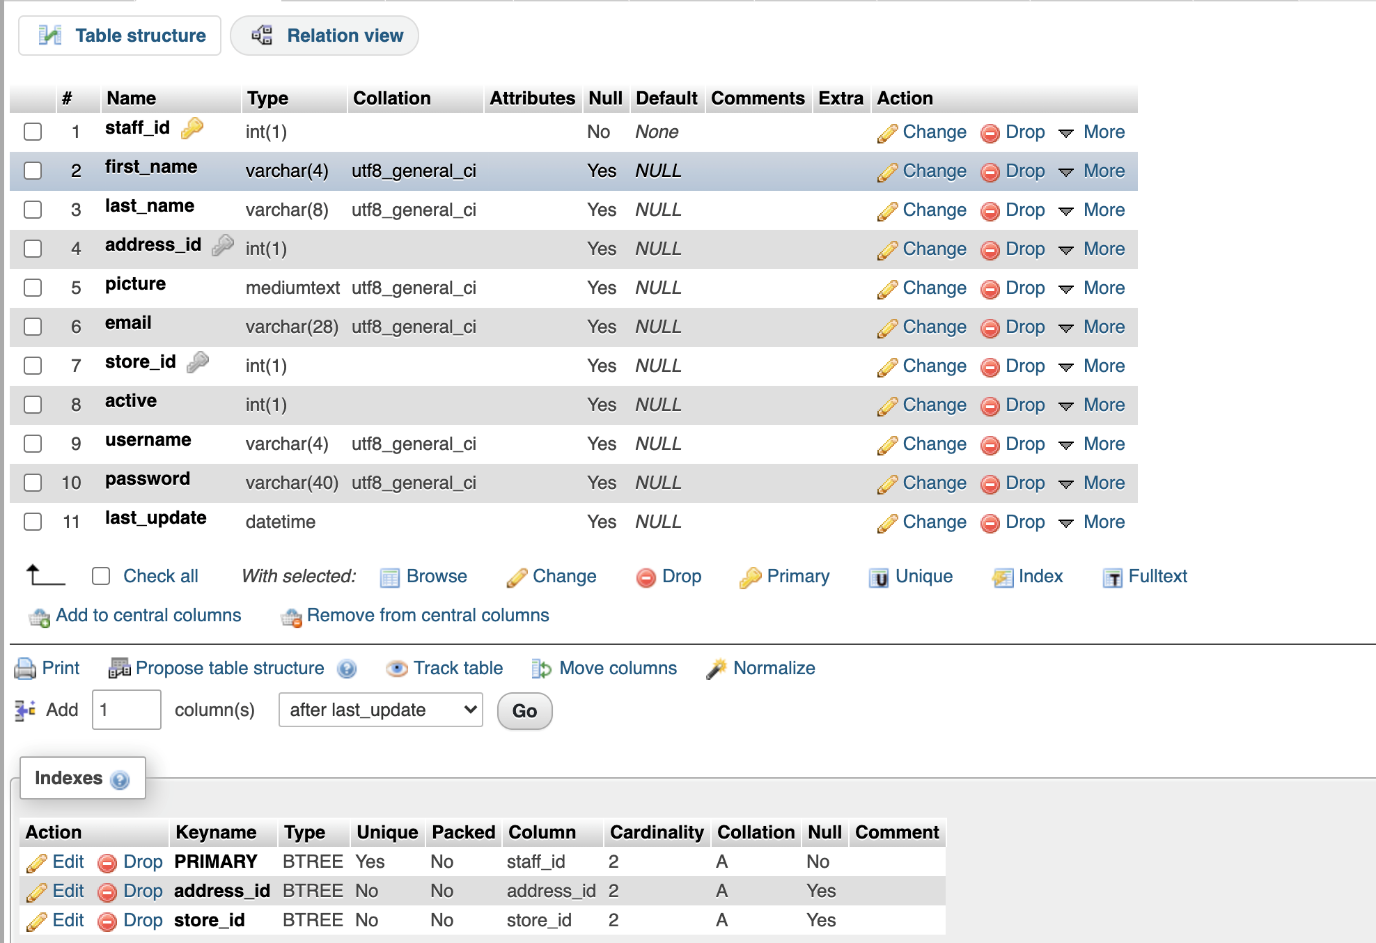
\includegraphics[width=\textwidth]{table_staff_struct}
		\caption{Structure of table "Staff"}	
	\end{figure}
	\begin{figure}[H]
		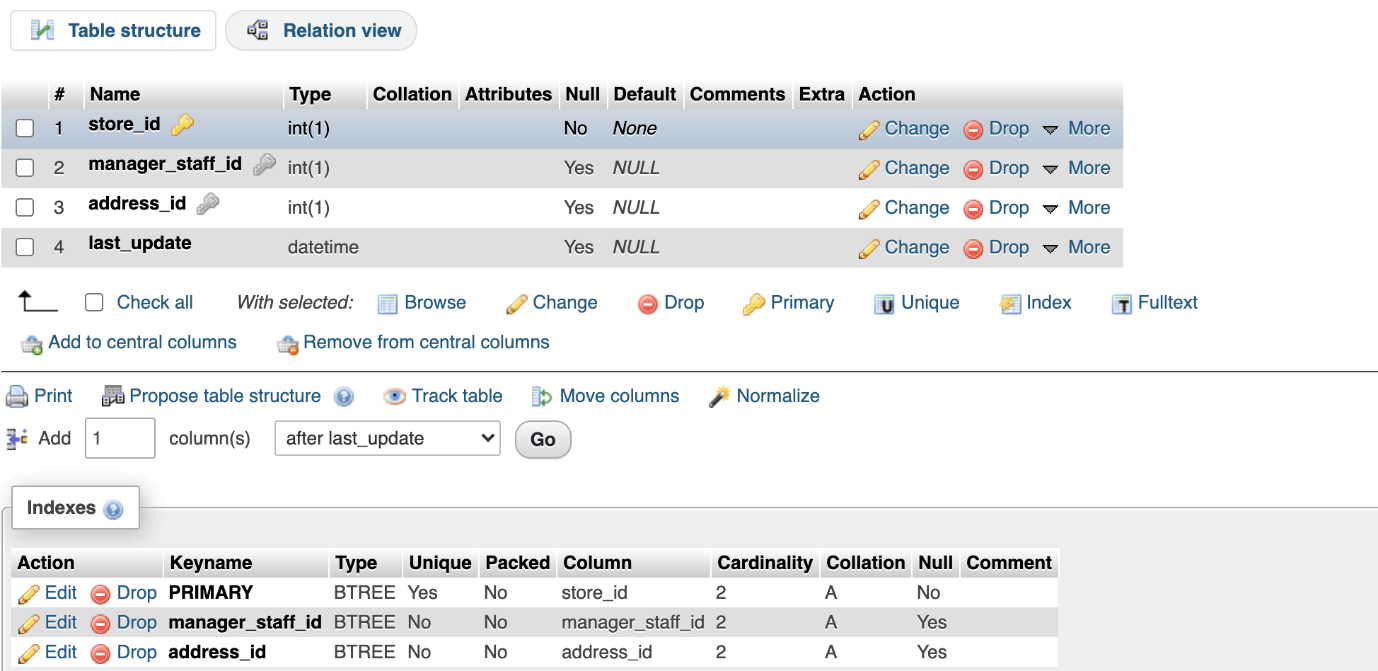
\includegraphics[width=\textwidth]{table_store_struct}
		\caption{Structure of table "Store"}	
	\end{figure}

\subsection{Final Results of Data Insertion \& Selection}
	\begin{figure}[H]
		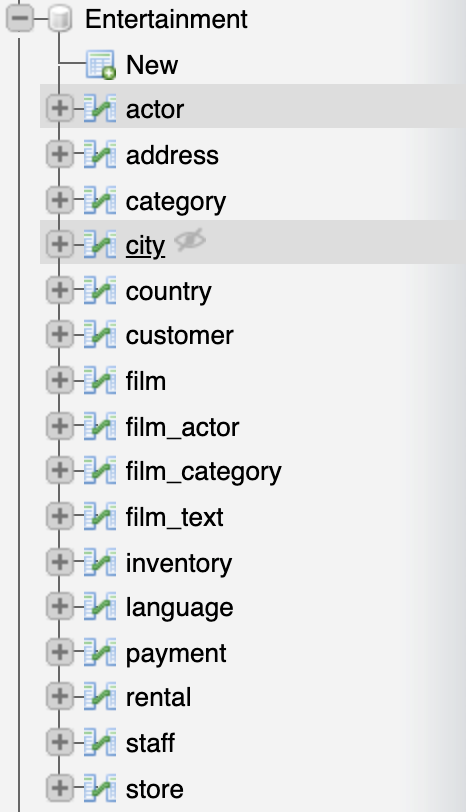
\includegraphics[width=\textwidth, height=\textheight, keepaspectratio]{data_insertion_selection}
	\end{figure}	

\subsection{Overview on Tables of Database "Entertainment"}
	\begin{figure}[H]
		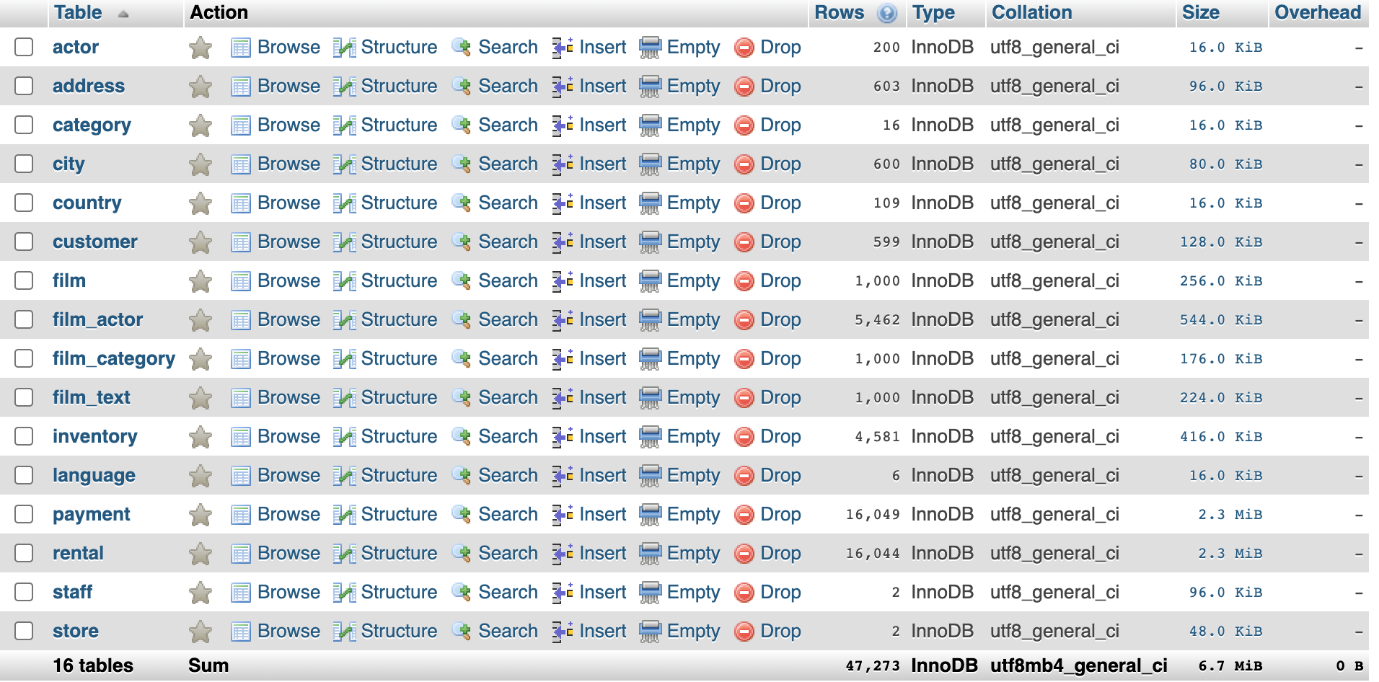
\includegraphics[width=\textwidth]{table_overview}
		\caption{Summary of tables within the database.}
	\end{figure}	
	
	\subsubsection{Table Contents}
		\begin{figure}[H]
			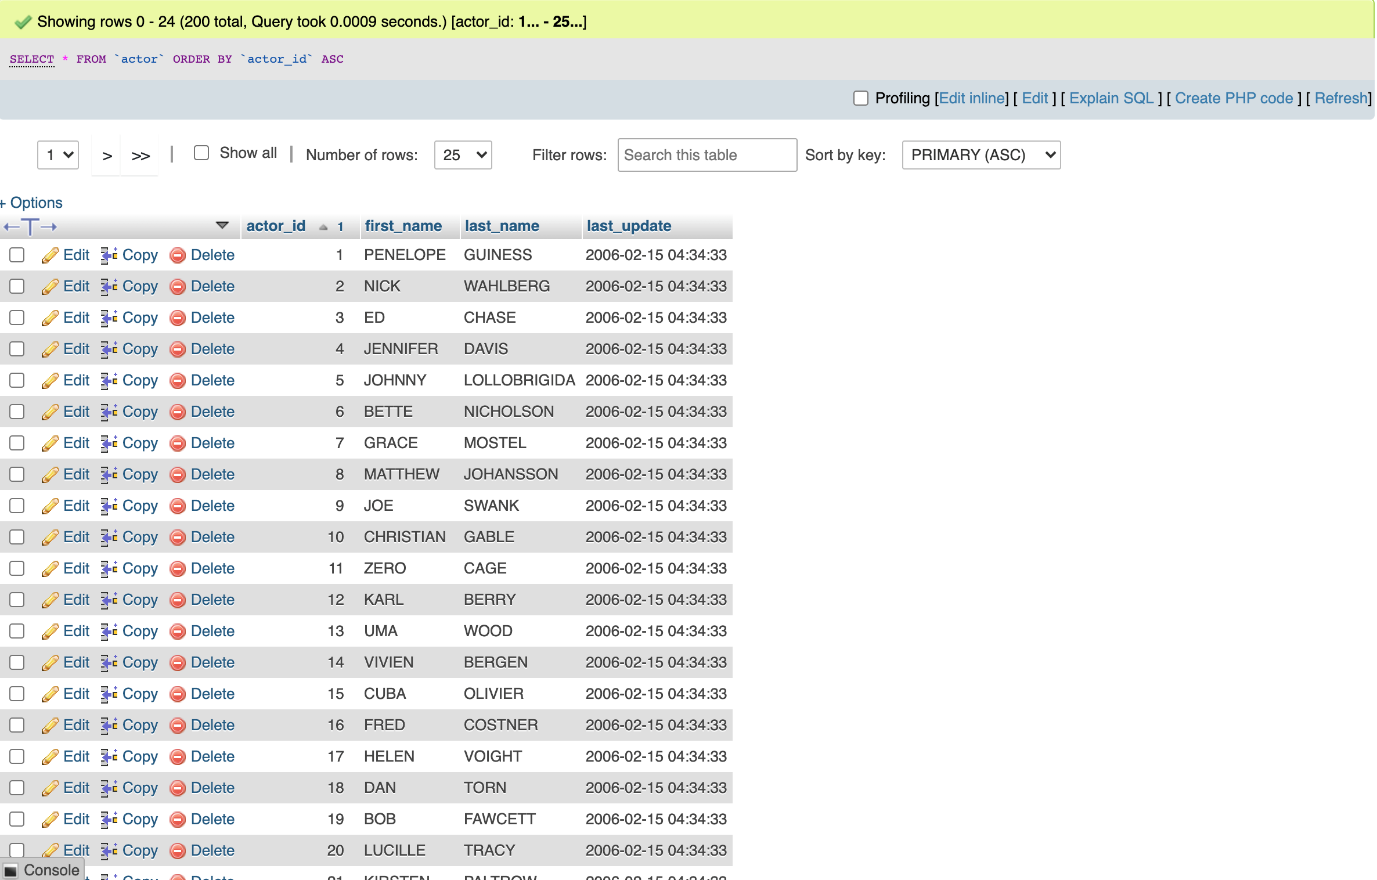
\includegraphics[width=\textwidth]{actor_content}
			\caption{Sample content of the table "Actor".}
		\end{figure}
		\begin{figure}[H]
			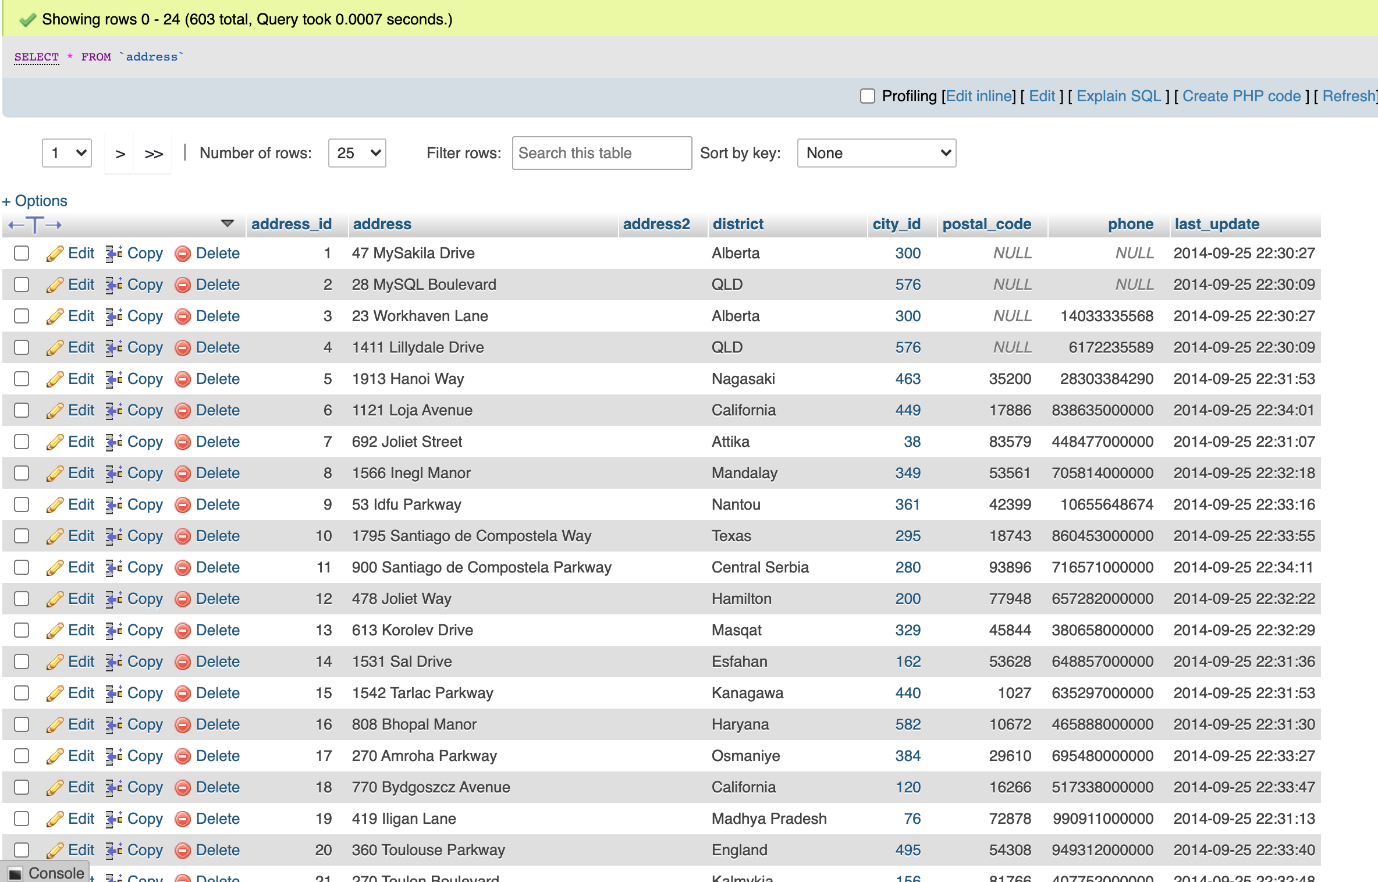
\includegraphics[width=\textwidth]{address_content}
			\caption{Sample content of the table "Address".}
		\end{figure}
		\begin{figure}[H]
			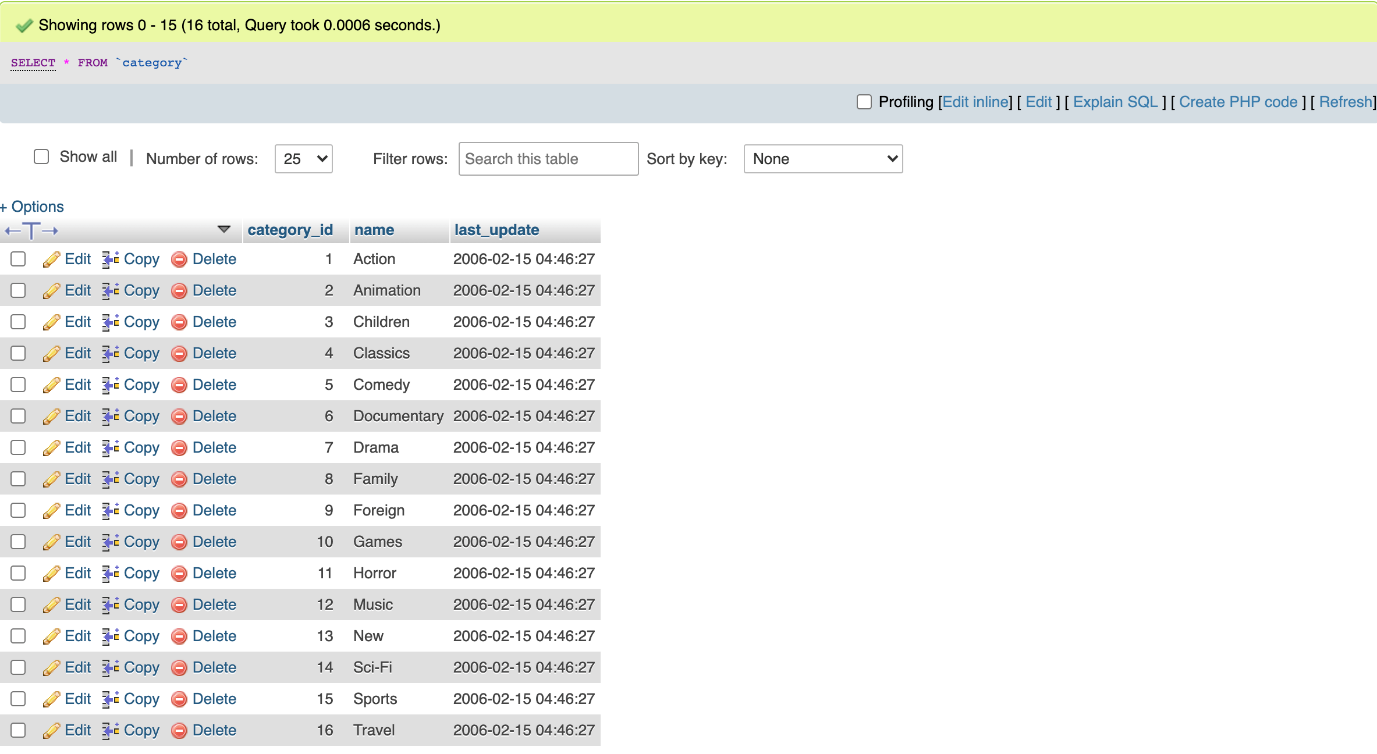
\includegraphics[width=\textwidth]{category_content}
			\caption{Sample content of the table "Category".}
		\end{figure}
		\begin{figure}[H]
			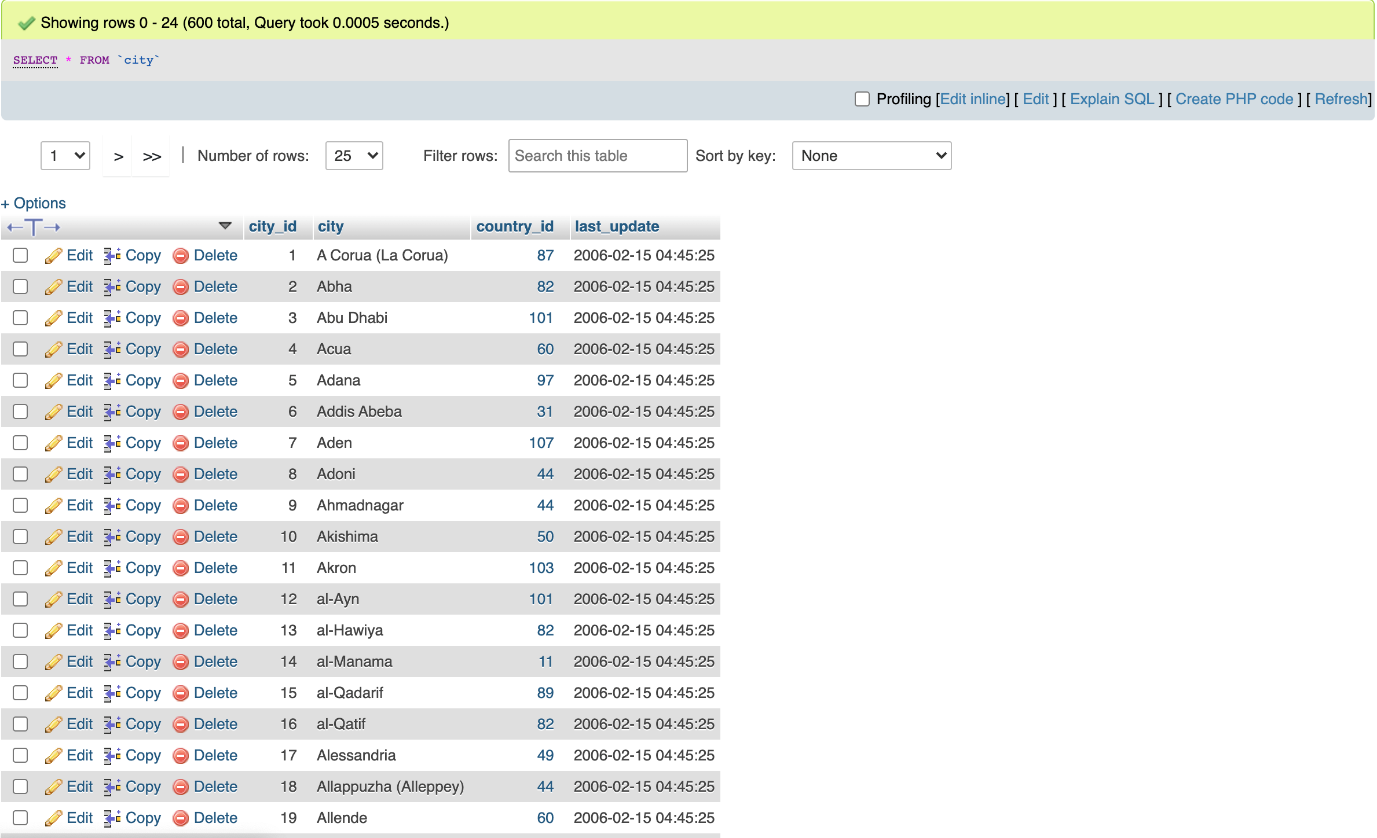
\includegraphics[width=\textwidth]{city_content}
			\caption{Sample content of the table "City".}
		\end{figure}
		\begin{figure}[H]
			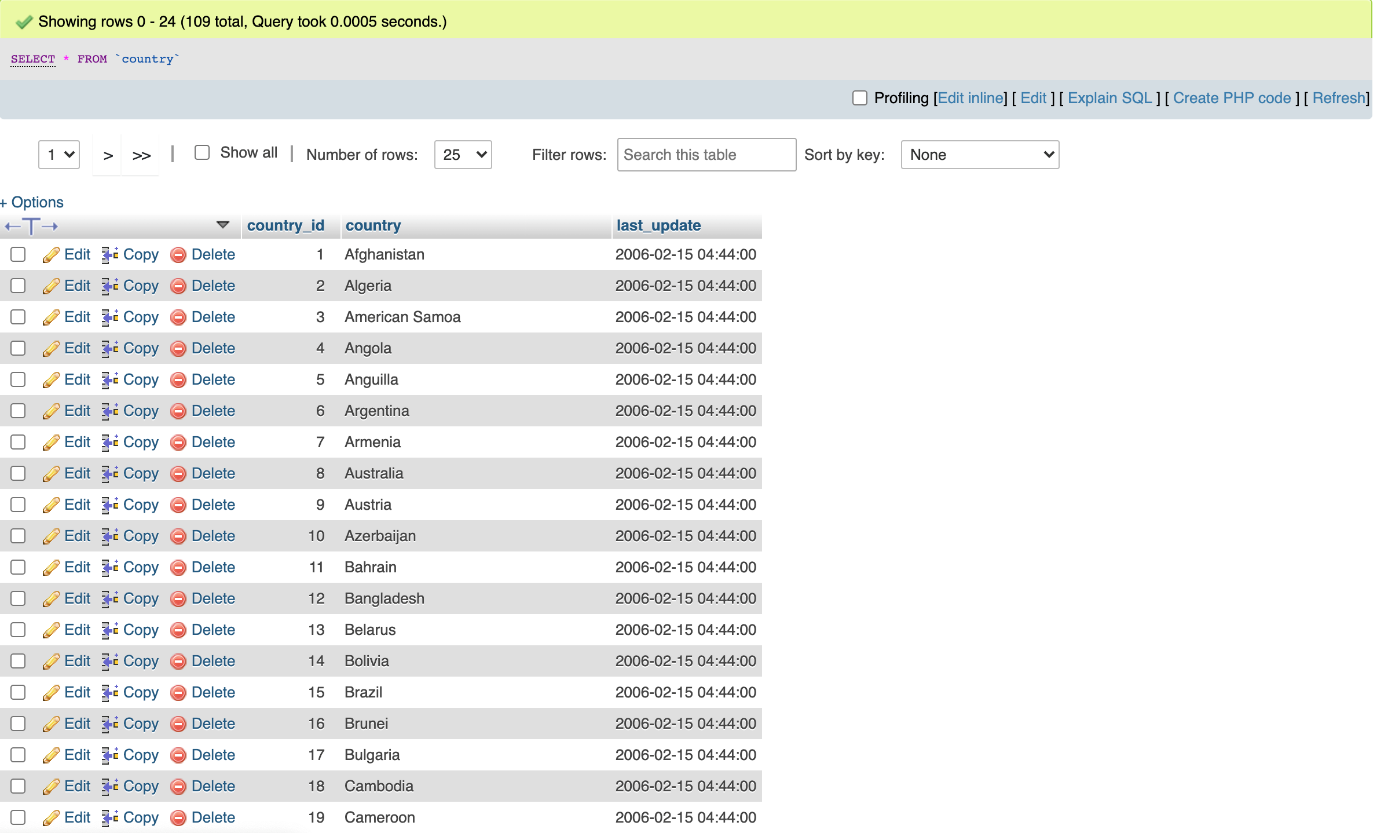
\includegraphics[width=\textwidth]{country_content}
			\caption{Sample content of the table "Country".}
		\end{figure}
		\begin{figure}[H]
			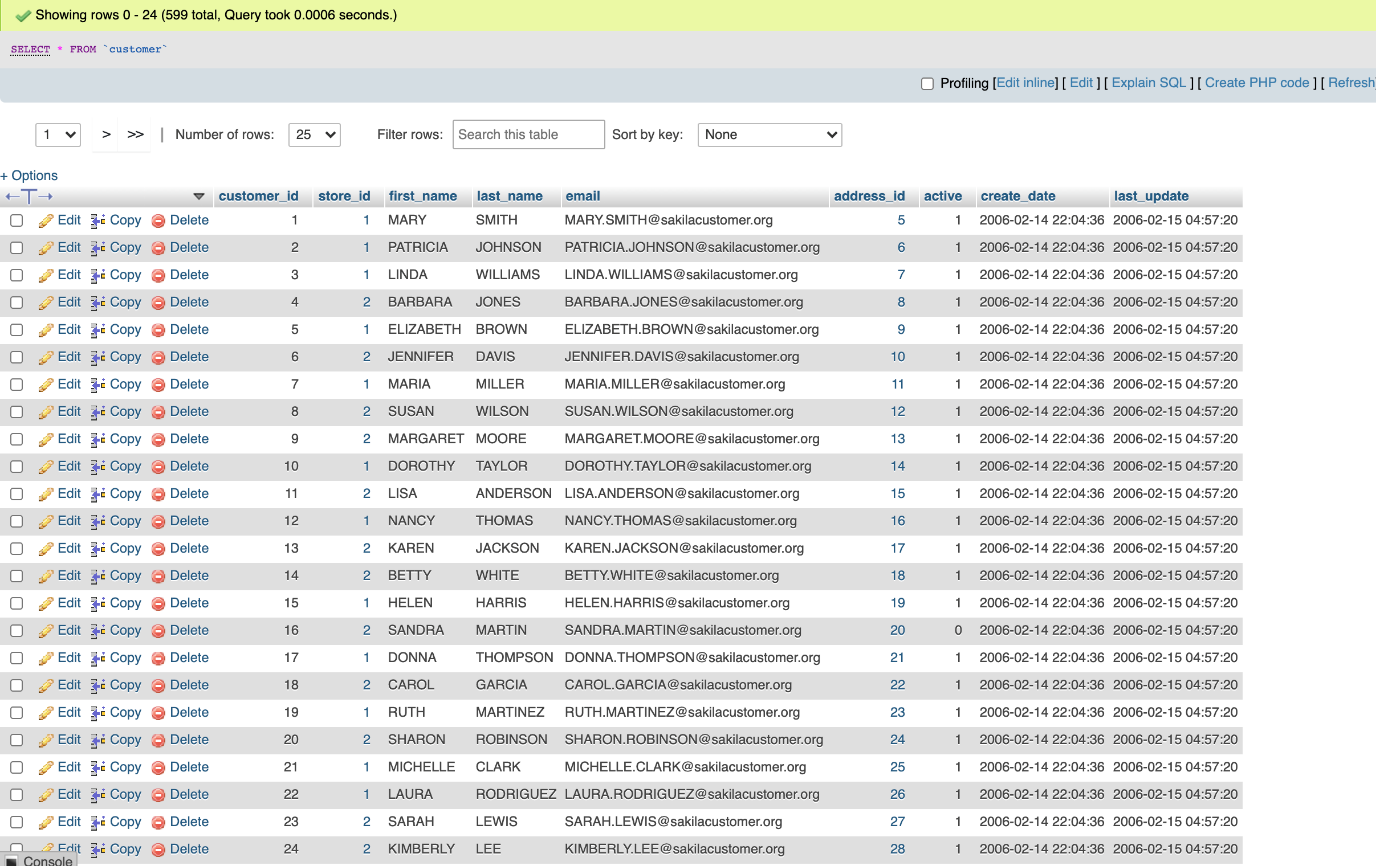
\includegraphics[width=\textwidth]{customer_content}
			\caption{Sample content of the table "Customer".}
		\end{figure}
		Amendment: The content of original\textunderscore language\textunderscore id is NULL throughout in the table "Film" as of the current iteration.
		\begin{figure}[H]
			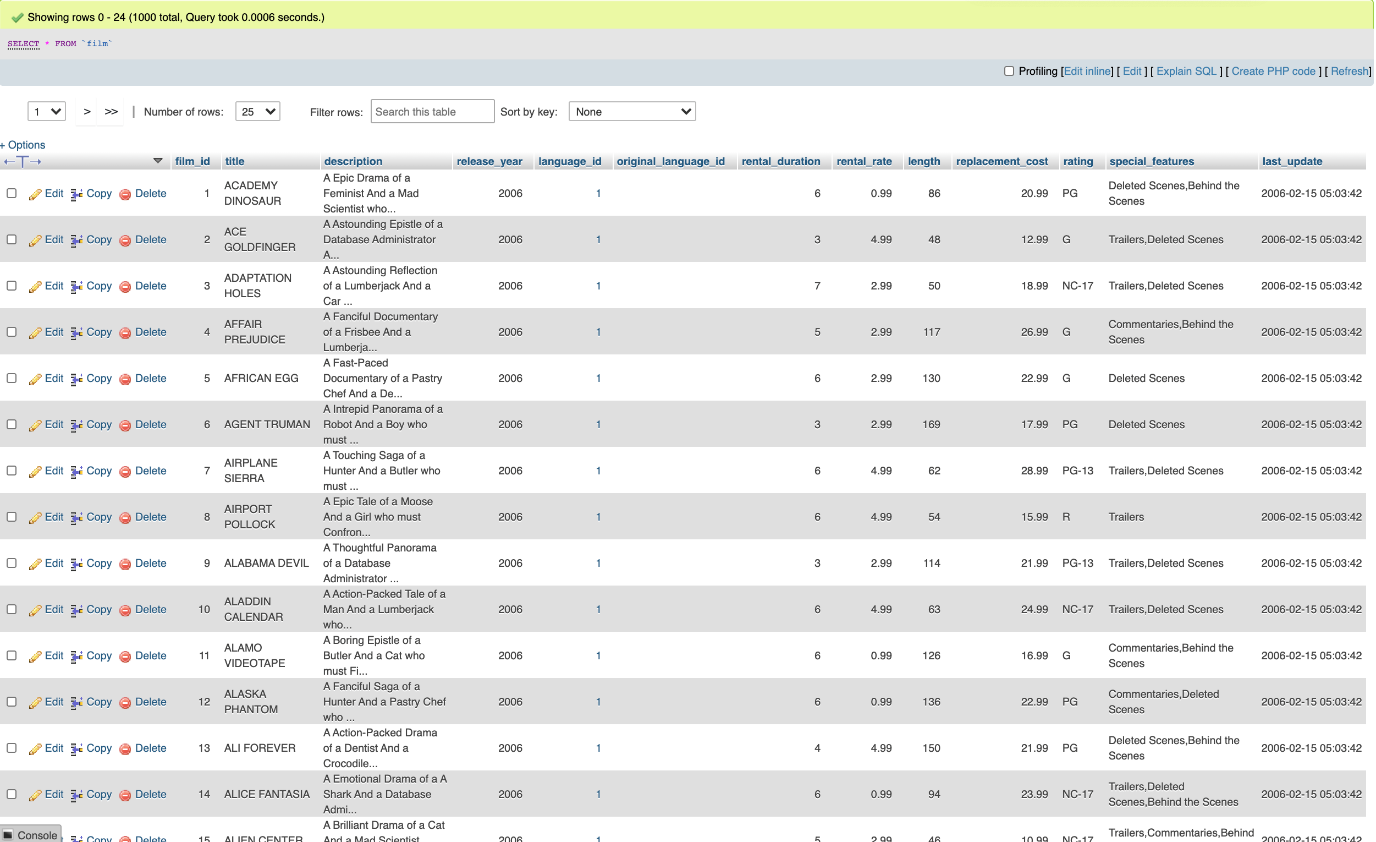
\includegraphics[width=\textwidth]{film_content}
			\caption{Sample content of the table "Film".}
		\end{figure}
		\begin{figure}[H]
			\includegraphics[width=\textwidth]{filmactor_content}
			\caption{Sample content of the table "Film\textunderscore Actor".}
		\end{figure}
		\begin{figure}[H]
			\includegraphics[width=\textwidth]{filmcategory_content}
			\caption{Sample content of the table "Film\textunderscore Category".}
		\end{figure}
		\begin{figure}[H]
			\includegraphics[width=\textwidth]{filmtext_content}
			\caption{Sample content of the table "Film\textunderscore Text".}
		\end{figure}
		\begin{figure}[H]
			\includegraphics[width=\textwidth]{inventory_content}
			\caption{Sample content of the table "Inventory".}
		\end{figure}
		\begin{figure}[H]
			\includegraphics[width=\textwidth]{language_content}
			\caption{Sample content of the table "Language".}
		\end{figure}
		\begin{figure}[H]
			\includegraphics[width=\textwidth]{payment_content}
			\caption{Sample content of the table "Payment".}
		\end{figure}
		\begin{figure}[H]
			\includegraphics[width=\textwidth]{rental_content}
			\caption{Sample content of the table "Rental".}
		\end{figure}
		\begin{figure}[H]
			\includegraphics[width=\textwidth]{staff_content}
			\caption{Sample content of the table "Staff".}
		\end{figure}
		\begin{figure}[H]
			\includegraphics[width=\textwidth]{store_content}
			\caption{Sample content of the table "Store".}
		\end{figure}

\subsection{Normalization}
	\subsubsection{Entity Relation Diagram After Normalization}
		\begin{figure}[H]
			\includegraphics[width=\textwidth]{er_normalized}
			\caption{Database structure after normalization.}
		\end{figure}

	\subsubsection{Tables Affected by Normalization}
		The tables Film\textunderscore Special\textunderscore Features is normalized from the Film table to preserve compliance with the First Normal Form. 
		\begin{figure}[H]
			\includegraphics[height = \textheight]{table_filmspecialfeatures_norm}
			\caption{Table "Film\textunderscore Special\textunderscore Features", normalized.}
		\end{figure}

		The District, City and Address tables have been recompiled after normalization. \\\\
		The field last\textunderscore update is retained for the purpose of easing maintenance of the altered tables. \\\\
		It can be noted that for the Address and City tables, many errors within the database have been uncovered due to the use of normalization that otherwise would have gone unnoticed.  Errors found include: 
		\begin{itemize}
			\item Cities with ID 121, 493 and 583 not having a listed district. Their district\textunderscore id fields in the newly reorganized City table have been left blank.
			\item Entry with city\textunderscore id 313 in the City table not existing within the address table. district\textunderscore id field of this city also left blank in the City table.
			\item Multiple occurences of the same city\textunderscore id being in multiple districts in the address table. To preserve database integrity after normalization, one of the extra districts is removed with the use of an SQL command containing the GROUP BY keyword. 
		\end{itemize}
		\begin{figure}[H]
			\includegraphics[width=\textwidth]{table_district_norm}
			\caption{Table "District", normalized.}
		\end{figure}
		\begin{figure}[H]
			\includegraphics[width=\textwidth]{table_address_norm}
			\caption{Table "Address", normalized.}
		\end{figure}
		\begin{figure}[H]
			\includegraphics[width=\textwidth]{table_city_norm}
			\caption{Table "City", normalized.}
		\end{figure} 
		Note that \textbf{original\textunderscore film\textunderscore id} now has a foreign key relation with the Language table to increase consistency. Its database has consequently been coverted to \textbf{int}.
		\begin{figure}[H]
			\includegraphics[width=\textwidth]{table_film_norm}
			\caption{Table "Film", normalized.}
		\end{figure}
		\begin{figure}[H]
			\includegraphics[height = 20cm]{table_filmrental_norm}
			\caption{Table "Film\textunderscore Rental", normalized.}
		\end{figure}
		\begin{figure}[H]
			\includegraphics[width=\textwidth]{table_staff_norm}
			\caption{Table "Staff", normalized.}
		\end{figure}
		\begin{figure}[H]
			\includegraphics[width=\textwidth]{table_stafflogin_norm}
			\caption{Table "Staff\textunderscore Login", newly created after normalization.}
		\end{figure}


	\subsubsection{Table Structures After Normalization}
		\begin{figure}[H]
			\includegraphics[width=\textwidth]{table_district_nstruct}
			\caption{Structure of table "District", normalized.}
		\end{figure}
		\begin{figure}[H]
			\includegraphics[width=\textwidth]{table_film_nstruct}
			\caption{Structure of table "Film", normalized.}
		\end{figure}
		\begin{figure}[H]
			\includegraphics[width=\textwidth]{table_filmtext_nstruct}
			\caption{Structure of table "Film\textunderscore Text", normalized.}
		\end{figure}
		\begin{figure}[H]
			\includegraphics[width=\textwidth]{table_staff_nstruct}
			\caption{Structure of table "Staff", normalized.}
		\end{figure}
		\begin{figure}[H]
			\includegraphics[width=\textwidth]{table_stafflogin_nstruct}
			\caption{Structure of table "Staff\textunderscore Login", normalized.}
		\end{figure}
	
	\subsubsection{Foreign Key Relations After Normalization}
		To preserve the integrity of relations inside of the database, foreign key constraints within the database have been modified based on these criterion:
		\begin{itemize}
			\item Two foreign keys have been modified with ON DELETE CASCADE as the deletion of table data involving these foreign keys will only affect this one table, and will not cascade down the entire database. The tables involved are "Film\textunderscore Actor" and "Film\textunderscore Category", which have their primary keys in the tables "Actor" and "Category" respectively. 
			\item The primary keys of three tables are left with the original ON DELETE RESTRICT constraint as these tables are central components of the entire database, and should have all deletions resolved on lower levels on the database before they themselves are allowed to be deleted. This affects all tables having a foreign key from the tables "Customer", "Film", and "Staff".
			\item Every other foreign key constraint is set to ON DELETE SET NULL by default. This is to facilitate easy reorganisation and maintenance on the database as this database contains numerous errata; having the ability to delete erroneous entries easily drastically improves the ease of managing and fixing the database.
			\item For the same reasons as above, all foreign key constraints with regards to updates have been set to ON UPDATE CASCADE. This is to accomodate the many value changes and error corrections that are expected to take place over the course of using this database. 
		\end{itemize}
		Displayed below are examples of affected foreign key relations.
		\begin{figure}[H]
			\includegraphics[width=\textwidth]{actor_cascade}
			\caption{The table "Film\textunderscore Actor" having its ON DELETE relation with "Actor" modified to CASCADE.}
		\end{figure}
		\begin{figure}[H]
			\includegraphics[width=\textwidth]{category_cascade}
			\caption{The table "Film\textunderscore Category" having its ON DELETE relation with "Category" modified to CASCADE.}
		\end{figure}
		\begin{figure}[H]
			\includegraphics[width=\textwidth]{customer_restrict}
			\caption{The table "Rental" having its ON DELETE relation with "Customer" modified to RESTRICT.}
		\end{figure}
		\begin{figure}[H]
			\includegraphics[width=\textwidth]{address_restrict}
			\caption{The table "Store" having its ON DELETE relation with "Address" modified to RESTRICT.}
		\end{figure}
		\begin{figure}[H]
			\includegraphics[width=\textwidth]{store_restrict}
			\caption{The table "Staff" having its ON DELETE relation with "Store" modified to RESTRICT.}
		\end{figure}
		\begin{figure}[H]
			\includegraphics[width=\textwidth]{film_restrict}
			\caption{The table "Film\textunderscore Text" having its ON DELETE relation with "Film" modified to RESTRICT.}
		\end{figure}
		\begin{figure}[H]
			\includegraphics[width=\textwidth]{table_film_norm_fk}
			\caption{A foreign key relation between original\textunderscore language\textunderscore id and the table "Language" has also been applied.}
		\end{figure}
		\begin{figure}[H]
			\includegraphics[width=\textwidth]{staff_restrict}
			\caption{The table "Payment" having its ON DELETE relation with "Staff" modified to RESTRICT.}
		\end{figure}
		\begin{figure}[H]
			\includegraphics[width=\textwidth]{setnull_cascade}
			\caption{The default setting for foreign key relations with other tables in this database.}
		\end{figure}

	\subsubsection{Insertion After Normalization}
		\begin{figure}[H]
			\includegraphics[width=\textwidth, height=\textheight, keepaspectratio]{specialfeatures11_insert}
			\caption{Insertion of new data into the table "Film\textunderscore Special\textunderscore Features" after normalization}
		\end{figure}
		\begin{figure}[H]
			\includegraphics[width=\textwidth, height=\textheight, keepaspectratio]{filmrental_insert_norm}
			\caption{Insertion of new data into the table "Film\textunderscore Rental" after normalization}
		\end{figure}
		\begin{figure}[H]
			\includegraphics[width=\textwidth, height=\textheight, keepaspectratio]{address_insert_norm}
			\caption{Insertion of new data into the table "Address" after normalization}
		\end{figure}
		\begin{figure}[H]
			\includegraphics[width=\textwidth, height=\textheight, keepaspectratio]{film_insert_norm}
			\caption{Insertion of new data into the table "Film" after normalization}
		\end{figure}
		\begin{figure}[H]
			\includegraphics[width=\textwidth, height=\textheight, keepaspectratio]{customer1_insert_norm}
			\caption{Insertion of new data into the table "Customer" after normalization}
		\end{figure}
		\begin{figure}[H]
			\includegraphics[width=\textwidth, height=\textheight, keepaspectratio]{district1_insert_norm}
			\caption{Insertion of new data into the table "District" after normalization}
		\end{figure}
		\begin{figure}[H]
			\includegraphics[width=\textwidth]{city1_insert_norm}
			\caption{Insertion of new data into the table "City" after normalization}
		\end{figure}
		\begin{figure}[H]
			\includegraphics[width=\textwidth]{staff1_insert_norm}
			\includegraphics[width=\textwidth]{staff2_insert_norm}
			\caption{Insertion of new data into the table "Staff" after normalization}
		\end{figure}
		\begin{figure}[H]
			\includegraphics[width=\textwidth]{stafflogin1_insert_norm}
			\includegraphics[width=\textwidth]{stafflogin2_insert_norm}
			\caption{Insertion of new data into the table "Staff\textunderscore Login" after normalization}
		\end{figure}

	\subsubsection{Deletion After Normalization}
		Due to repurposing of Staff IDs into an Auto Incremented Primary Key, the following deletions were made to bring all the tables into consistency.
		\begin{figure}[H]
			\includegraphics[width=\textwidth]{staff1_delete_norm}
			\includegraphics[width=\textwidth]{staff2_delete_norm}
			\caption{Data deletion from the table "Staff" after normalization}
		\end{figure}
		\begin{figure}[H]
			\includegraphics[width=\textwidth]{stafflogin1_delete_norm}
			\includegraphics[width=\textwidth]{stafflogin2_delete_norm}
			\caption{Data deletion from the table "Staff\textunderscore Login" after normalization}
		\end{figure}

	\subsubsection{Updates After Normalization}
		\begin{figure}[H]
			\includegraphics[width=\textwidth]{stafflogin1_update_norm}
			\includegraphics[width=\textwidth]{stafflogin2_update_norm}
			\caption{Update on the table "Staff\textunderscore Login" after normalization}
		\end{figure}

\subsection{Selections Based on Original Database Using the WHERE Keyword} 
		\begin{figure}[H]
			\includegraphics[height = 16cm]{customer_selectwhere}
			\caption{Table "Customer"}
		\end{figure}
		\begin{figure}[H]
			\includegraphics[height = 16cm]{film_selectwhere}
			\caption{Table "Film"}
		\end{figure}
		\begin{figure}[H]
			\includegraphics[height = 16cm]{filmcategory_selectwhere}
			\caption{Table "Film\textunderscore Category"}
		\end{figure}
		\begin{figure}[H]
			\includegraphics[width=\textwidth]{inventory_selectwhere}
			\caption{Table "Inventory"}
		\end{figure}
		\begin{figure}[H]
			\includegraphics[width=\textwidth]{payment_selectwhere}
			\caption{Table "Payment"}
		\end{figure}

\newpage
\section{Report Part C}

\subsection{Website Link}
	\begin{center}
		\href{http://hcytt1.mercury.nottingham.edu.my/address.php}{Link to the Mercury Website}
	\end{center}

\subsection{Website Video Showcase}
	\begin{center}
		\href{https://numcmy-my.sharepoint.com/:v:/g/personal/hcycl3_nottingham_edu_my/EXSHVn9W0NpKs46qVvkPRaYB7jFJyir5uJE3W_kIAa8p0g?e=dCDxFW}{Link to Demonstration Video (OneDrive)}
	\end{center}

\subsection{Github Repository Link}
	\begin{center}
		\href{https://github.com/HolyKritGrenade/comp1044dbi_cw2webcode}{Link to Webcode}
	\end{center}

\subsection{Website Features}
	The website includes multiple features to enhance the user experience of the website. Among these include:
	\begin{itemize}
		\item Basic insertion, update and deletion functionality
		\item Ability to search for specific database entries via any column via Selection
		\item No requirement for all data fields to be filled for updates
		\item Responsive website elements that will adapt to fit screens of any resolution and size
		\item Dropdown bar to ease transitioning between different tables
		\item Dialogs to report database status after any operation
		\item CSS design to enhance the visual appeal and increase fluidity of all website elements
	\end{itemize}
\subsection{Website Interface and Code Examples}
		\begin{figure}[H]
			\includegraphics[width=\textwidth, height=\textheight, keepaspectratio]{css}
			\caption{CSS code to design the website and ensure mobile compatibility.}
		\end{figure}
		\begin{figure}[H]
			\includegraphics[width=\textwidth]{Country (PC view)}
			\caption{Website view with a desktop monitor.}
		\end{figure}
		\begin{figure}[H]
			\includegraphics[width=\textwidth, height=\textheight, keepaspectratio]{Country (Mobile view)}
			\caption{Website view with a mobile device.}
		\end{figure}

\end{document}